\documentclass[12pt,a4paper]{report}

\usepackage[a4paper,margin=1in]{geometry}
\usepackage{graphicx}
\usepackage{amsmath}
\usepackage{amssymb}
\usepackage{booktabs}
\usepackage{algorithm}
\usepackage{algpseudocode}
\usepackage{hyperref}
\usepackage{times}
\usepackage{tikz}
\usetikzlibrary{shapes.geometric, arrows.meta, positioning}
\usepackage{float}
\usepackage[skip=4pt]{caption}
\usepackage{setspace}
\usepackage[htt]{hyphenat}

\setlength{\textfloatsep}{6pt plus 2pt minus 2pt}
\setlength{\intextsep}{6pt plus 2pt minus 2pt}
\setlength{\floatsep}{6pt plus 2pt minus 2pt}
\setlength{\abovecaptionskip}{3pt}
\setlength{\belowcaptionskip}{3pt}

\hypersetup{
    colorlinks=true,
    linkcolor=black,
    citecolor=black,
    urlcolor=blue,
    linktoc=all
}

\onehalfspacing

\begin{document}

\begin{titlepage}
    \centering
    \vspace*{0.8cm}
    {\large Université Marie et Louis Pasteur\par}
    {\large CNRS, institut FEMTO-ST\par}
    \vspace{0.3cm}
    {\large Master 2 --- Internet of Things (IoT)\par}
    \vspace{0.6cm}

    
\includegraphics[height=1.3cm,keepaspectratio]{logo-umlp.png}

    \vspace{0.6cm}

    {\Large \bfseries Master's Thesis\par}
    \vspace{0.8cm}

    \rule{\linewidth}{0.5pt}\par
    \vspace{0.5cm}
    {\huge \bfseries From Distributed Neural Networks to Quantized 3D Convolutional Networks for Shape Recognition on Programmable Matter\par}
    \vspace{0.5cm}
    \rule{\linewidth}{0.5pt}\par
    \vspace{1.4cm}

    {\large\itshape Georges Chaiban\par}
    \vspace{1.4cm}

    \begin{flushleft}
        \large
        \textbf{Internship supervisor:} Dr. Jad Bassil\\
        \textbf{Host laboratory:} Institut FEMTO-ST, Montbéliard\\
        \textbf{Internship period:} 1 February -- 31 July\\
    \end{flushleft}

    \vfill
    {\large 18 August 2026\par}
\end{titlepage}

\pagenumbering{roman}

\chapter*{Abstract}
\addcontentsline{toc}{chapter}{Abstract}

Programmable Matter (PM) systems are composed of many resource-constrained modules that must sense, compute, and coordinate locally, without relying on centralized infrastructure or a global view of the structure they form. A central open question for such systems is whether meaningful intelligence here, the ability of an assembled structure to recognize its own shape can run entirely on-module, under per-block memory and communication budgets measured in kilobytes. Prior work by Piranda et al. demonstrated that a distributed Artificial Neural Network (ANN) can be mapped as message-passing agents directly onto a BlinkyBlocks platform, letting a 256-block grid recognize its own shape among three simple 2D shapes. This thesis documents an internship carried out at institut FEMTO-ST that set out to extend this result toward better 3D shape recognition while keeping every model deployable on real BlinkyBlocks hardware. The work proceeded through six successive architectures: an int8-quantized reproduction of Piranda et al.'s original 2D ANN; a naive extension of that flat ANN to a 16$\times$16$\times$16 3D occupancy grid; a 2D Convolutional Neural Network (CNN) using local, face-neighbor message passing; a 3D CNN relying on a hardcoded height-map projection; a fully embedded 3D CNN with no hardcoded roles; and finally a Deep Embedded 3D CNN with three convolutional phases, compressed with TinyML int8 weight quantization. Each stage is evaluated in the VisibleSim simulator using message counts, confidence, and classification accuracy, exposing precisely why each design was replaced by the next: the flat 3D ANN's message count grew into the millions, while the final quantized model, validated on real BlinkyBlocks hardware, reached an overall accuracy of 88.0\% across six shape classes with a 3.77x reduction in weight-storage size. This thesis reports the full comparative results across all six stages and discusses the extent to which the final contribution resolves the problem stated at the outset.

\vspace{1cm}
\noindent\textbf{Keywords:} Programmable Matter, Distributed Neural Networks, TinyML, Model Quantization, BlinkyBlocks, Convolutional Neural Networks

\chapter*{Acknowledgements}
\addcontentsline{toc}{chapter}{Acknowledgements}

I would like to thank my internship supervisor, Dr. Jad Bassil, for their guidance throughout this project at institut FEMTO-ST. I am also grateful to Pr. Abdallah Makhoul, and Pr. Benoit Piranda, who collaborated through the whole internship of this work. Finally, I thank Dr. Jacques Bahi for making this internship fundable and possible.

\clearpage
\tableofcontents
\clearpage
\listoffigures
\clearpage
\listoftables

\clearpage
\pagenumbering{arabic}
\setcounter{page}{1}

\chapter{Introduction}

\section{Context and Background}

Programmable Matter systems are built from large numbers of physically identical modules that compute using only local, face-adjacent connections to their immediate neighbors. No module has a global view of the structure it is part of, and no central server coordinates the group: every decision the assembled structure makes, including something as basic as recognizing its own shape, has to emerge from purely local computation and purely local message exchange. This makes shape recognition a natural benchmark problem for testing whether meaningful intelligence can run entirely on-module, since a correct answer requires every block to contribute a small piece of information that only becomes meaningful once aggregated with the rest of the structure.

The BlinkyBlocks platform, developed at institut FEMTO-ST, is one such Programmable Matter system, made of physical cubic modules that snap together face-to-face, each carrying its own microcontroller, a small amount of RAM and flash memory, colored LEDs for visual feedback, and short-range communication links to its up-to-six face-connected neighbors. Because each module carries only a few kilobytes of memory, any model deployed on BlinkyBlocks has to be fully distributed, computed collaboratively across all modules via message passing, and small enough in weight-storage to fit within a single module's flash memory, alongside the firmware that runs the rest of the platform's functionality (lattice self-assembly, motion planning, communication stack, and so on). These two constraints, distribution and footprint, run through every design decision documented in this thesis.

Alongside the real hardware, this work makes heavy use of VisibleSim, a simulator for modular robots. VisibleSim executes the exact same C/C++ firmware that would run on physical BlinkyBlocks, simulating the message-passing network, per-module timing, and 3D visualization, which makes it possible to iterate on a distributed algorithm's correctness and communication cost long before committing to a real hardware test. Every architecture presented in this thesis was first validated in VisibleSim before any hardware deployment was attempted.

\section{Problem Statement}

Piranda et al.~\cite{piranda2024ai4pm} demonstrated that a distributed Artificial Neural Network can be mapped directly onto a BlinkyBlocks platform as a collection of message-passing agents, letting a 256-block grid recognize its own shape among three simple 2D silhouettes (square, disk, triangle) with only 552 bytes of memory per block, and with classification results matching those of an equivalent centralized ANN run offline. This result established the core feasibility claim this thesis builds on, which is that a neural network can be executed in a fully distributed manner across BlinkyBlocks modules, with each block's local computation and local messages together reconstructing what a single centralized network would have computed.

However, Piranda et al.'s architecture is a flat, fully-connected network. He showed that every input pixel is wired to every hidden-layer neuron, and every hidden neuron is wired to every output class. This design was adequate for a small, fixed 16$\times$16 grid and three simple 2D shape classes, but it does not scale well in two directions that matter for any realistic Programmable Matter deployment. First, extending a flat fully-connected architecture to volumetric 3D shapes multiplies the input size by the third spatial dimension, which, as this thesis demonstrates concretely in Chapter~\ref{ch:methodology}, causes the number of exchanged messages to explode by orders of magnitude, since every module's local input layer still has to fan out to every hidden neuron via message passing rather than through a genuinely local operation. Second, more shape classes require deeper, higher-capacity models, and a deeper flat network grows its weight count and therefore its BlinkyBlocks flash footprint multiplicatively rather than gracefully.

The problem this internship set out to address is as follows: First, we have to find a distributed architecture that classifies a richer set of volumetric 3D shapes without the flat ANN's combinatorial blow-up in message count, and second, we should ensure that whatever model results from that search can actually be compressed to fit within a real BlinkyBlock's flash memory budget, since a model that only exists as a VisibleSim simulation delivers none of Programmable Matter's practical promise.

These two constraints pull in partially opposing directions, which is what makes the problem non-trivial rather than a straightforward engineering exercise. Increasing a model's capacity to recognize more shape classes, or to recognize shapes under a wider range of size, position, and orientation variation generally requires more parameters, which directly threatens the second problem, yet reducing a model's capacity to stay safely within a fixed memory budget generally reduces its ability to satisfy the first problem. Piranda et al.'s original architecture sits at one extreme of this trade-off: it is small enough to fit comfortably within 552 bytes per block, but only because its 3-class, fixed-2D-grid task is narrow enough not to require more capacity than that. Simply scaling that same architecture up, as Stage~2 of this thesis's methodology does directly, shows that the naive way of adding capacity (a larger fully-connected input layer) fails the first problem in a different way, not through a memory-budget violation but through a communication-cost explosion, before it ever gets close to violating the second problem. Navigating between these two failure modes, rather than falling into either one, is the central technical challenge addressed across the six stages of Chapter~\ref{ch:methodology}.

\section{Objectives and Contributions}

The objective of this internship was to design, implement, and validate, first in simulation and then on real hardware, a distributed neural architecture capable of classifying a richer vocabulary of 3D shapes than Piranda et al.'s original work, while remaining deployable within BlinkyBlocks' memory constraints. Rather than arriving at this architecture directly, the work proceeded iteratively through six successive stages, each one exposing a specific limitation of its predecessor and motivating the next design change:

\begin{enumerate}
    \item An int8-quantized reproduction of Piranda et al.'s original 2D ANN, establishing a working baseline and a first hands-on exposure to weight quantization.
    \item A naive extension of that same flat ANN architecture to a 3D occupancy grid, which exposed the message-count explosion problem described above.
    \item A 2D Convolutional Neural Network (CNN) using local computation and face-neighbor message passing, re-tested on Piranda et al.'s original 2D task to directly measure the efficiency gained by convolution.
    \item A 3D CNN built on top of a hardcoded height-map projection, which extended the 2D CNN's efficiency to 3D shapes but reintroduced a structural limitation: only a fixed subset of blocks performed the projection role.
    \item An Embedded 3D CNN in which every block in the assembled structure participates in inference directly, with no hardcoded positions or privileged roles.
    \item A Deep Embedded 3D CNN with three convolutional phases (one additional message-passed layer beyond stage 5), classifying six shape classes, and compressed with TinyML int8 weight quantization to fit BlinkyBlocks flash memory.
\end{enumerate}

The final contribution of this thesis is this sixth-stage model: a distributed 3D CNN validated both in VisibleSim and on real BlinkyBlocks hardware, achieving an overall accuracy of 88.0\% across six shape classes with a 3.77x reduction in weight-storage size relative to its unquantized float32 form. Equally important as this final result is the comparative evidence gathered across all six stages, presented in Chapter~\ref{ch:results}, which makes explicit why each earlier design was abandoned and quantifies, stage by stage, the efficiency and accuracy trade-offs involved.

Each of the six stages listed above corresponds to a specific, falsifiable hypothesis about what limitation the previous stage suffered from, and each stage's VisibleSim evaluation (Chapter~\ref{ch:methodology}) was designed specifically to confirm or refute that hypothesis rather than simply to report a single overall accuracy figure. Stage~2's hypothesis was that a flat architecture's message cost would scale poorly with 3D grid size; Stage~3's was that convolution would recover most of that lost efficiency without sacrificing accuracy on Piranda et al.'s original task; Stage~4's was that a hardcoded projection could extend that efficiency to 3D shapes, at the cost of an orientation dependency; Stage~5's was that removing the hardcoded projection entirely, letting every block participate, would both resolve that dependency and keep message cost proportional to structure size; and Stage~6's was that this same design could be safely deepened and widened to a richer shape vocabulary once quantized for real hardware. Presenting the work this way, as a sequence of hypotheses tested against measured evidence rather than as a single architecture presented without its rejected alternatives, is intended to make the reasoning behind the final design auditable: a reader who doubts that Stage~6's architecture was the right choice can trace, stage by stage, the specific evidence that ruled out each simpler alternative.

\section{Thesis Organization}

The remainder of this thesis is organized as follows. Chapter~\ref{ch:sota} reviews the state of the art in distributed intelligence on modular robots and in embedded model compression. Chapter~\ref{ch:context} describes the internship's host institution, the BlinkyBlocks hardware platform, the VisibleSim simulator, and restates the problem in concrete technical terms. Chapter~\ref{ch:methodology} presents the methodology and the full technical detail of all six architectural stages, including the design, implementation, and VisibleSim results of each. Chapter~\ref{ch:results} consolidates the comparative results across all six stages and presents the final model's full VisibleSim and real-hardware evaluation. Chapter~\ref{ch:contribution} explicitly connects the final contribution back to the problem statement of Chapter~1. Chapter~\ref{ch:conclusion} concludes the thesis and discusses perspectives for future work.

\chapter{State of the Art}
\label{ch:sota}

\section{Programmable Matter and Self-Reconfigurable Modular Robots}

Programmable Matter refers to physical material or a physical system composed of many small, typically identical units, capable of changing its physical properties such as shape and density in response to user input, without requiring an external, centralized controller. Self-reconfigurable modular robot systems are the most mature physical realization of this concept: assemblies of identical robotic modules that can attach to, detach from, and move relative to their neighbors to change the overall shape of the assembly. Lattice-based systems, where modules occupy discrete positions on a regular 2D or 3D grid and only ever interact with their immediate lattice neighbors, are a particularly tractable subclass of this family, since the discreteness of the lattice makes both physical assembly and distributed algorithm design considerably simpler than in free-form or continuous modular systems. BlinkyBlocks, the platform used throughout this thesis, is a lattice-based cubic system: each module occupies one cell of a 3D grid and connects face-to-face with up to six neighbors.

A defining characteristic of these systems, and the one most relevant to this thesis, is the absence of any centralized computation or global information. Every module runs the same small program, senses only its immediate physical neighbors, and can only exchange messages with those same immediate neighbors. Any capability the assembled structure exhibits as a whole, from self-reconfiguration to shape recognition, must therefore be an emergent property of many identical, purely local computations combined through local message passing. This constraint shapes every architectural decision documented in this thesis: at no stage of the six-stage progression described in Chapter~\ref{ch:methodology} does any single block gain access to information about the whole structure except through the same local sensing-and-messaging mechanism available to every other block.

This absence of centralization is not merely a simplifying assumption but a direct consequence of the physical scale these systems are intended to reach. A Programmable Matter system envisioned at production scale might comprise thousands or millions of individual modules; a design that required even a single module to maintain a complete, up-to-date model of the whole structure would place an unbounded memory and communication burden on that module as the system grows, defeating the purpose of using many small, cheap, identical units in the first place. The alternative is the architecture this thesis adopts, which is to require every module to carry only $O(1)$ memory and to exchange only $O(1)$ messages per neighbor, regardless of how large the overall structure becomes, so that the system's total resource cost grows linearly with its size rather than combinatorially. Section~\ref{sec:stage2} of this thesis documents, concretely, what happens when an architecture violates this principle even slightly.

\section{The BlinkyBlocks Platform and VisibleSim Simulator}

BlinkyBlocks and VisibleSim, both developed at institut FEMTO-ST, form the specific lattice-based modular robot platform and companion simulator this thesis's six architectural stages were implemented, trained, and evaluated on; Chapter~\ref{ch:context} describes their technical specifications in the detail needed to understand this thesis's implementation choices, but it is worth situating them here, in the state-of-the-art context, as one instance of a broader family of cubic, lattice-based modular robot platforms studied in the self-reconfigurable robotics literature. What distinguishes BlinkyBlocks for the purposes of this thesis is not any single hardware feature but the combination of three properties: a rigid, discrete 3D lattice (which makes the ``local $3\times3\times3$ neighborhood'' notion central to every convolutional architecture in this thesis well-defined and physically meaningful), a face-adjacent communication topology (which is exactly the topology every message-passed convolution in this thesis is designed around), and a companion simulator, VisibleSim, capable of running the identical firmware intended for physical hardware. This last property is what allowed every one of the six stages documented in Chapter~\ref{ch:methodology} to be developed, debugged, and evaluated in simulation first, with only the final Stage~6 architecture actually committed to a real hardware deployment.

\section{Distributed Neural Networks on Modular Robots}

The starting point for this internship, and the work this thesis most directly extends, is Piranda et al.~\cite{piranda2024ai4pm}, ``AI4PM: Distributed and Intelligent Programmable Matter.'' That work demonstrated that a small Artificial Neural Network, with a flat, fully-connected architecture made of a 256-unit input layer, a 64-unit hidden layer, and a 3-unit output layer, could be mapped onto a 256-block BlinkyBlocks grid as a set of cooperating message-passing agents, rather than executed by any single centralized controller. Concretely, each of the 256 input-layer units corresponds to one cell of a 16$\times$16 2D grid (lit or unlit, depending on whether a BlinkyBlock is physically present at that position), each hidden-layer unit and output-layer unit is instantiated as a small agent capable of accumulating weighted contributions arriving as messages from the layer below it, and additional aggregation agents (in Piranda et al.'s terminology, Super Node and Divider agents) combine the many parallel local contributions into the network's final classification decision. The reported results showed that this fully distributed execution reproduces, output-for-output, what a centralized evaluation of the same trained network would have produced, while requiring only 552 bytes of memory per block, a figure that includes both the block's share of the network's weights and its runtime working memory.

This result is the foundation this thesis builds on, and Stage~1 of the methodology presented in Chapter~\ref{ch:methodology} begins by directly reproducing it, this time with int8 weight quantization applied. However, as argued in Section~1.2, the flat, fully-connected structure of Piranda et al.'s ANN is precisely what limits its applicability to richer shape vocabularies and to 3D volumetric shapes, since scaling a fully-connected layer to a larger input (a 3D grid rather than a 2D one) multiplies both its parameter count and, critically for a message-passing implementation, the number of messages required to propagate every input unit's contribution to every hidden unit. Stage~2 of this thesis's methodology makes this scaling problem concrete and measurable.

\section{Convolutional Approaches for Distributed Robotic Control}

Separately from the shape-recognition line of work, Dobreva et al.~\cite{dobreva} showed that convolutional architectures relying only on local, face-neighbor message passing can be used to directly control decentralized modular robots built from pivoting cubes, a different physical reconfiguration mechanism from BlinkyBlocks' static lattice assembly, but one that shares the same fundamental constraint of purely local sensing and communication. Their result is significant for this thesis for a structural reason rather than a shape-recognition reason: it demonstrates that convolution, as a computational pattern, composes naturally with the face-adjacent communication topology already native to lattice-based modular systems. A convolutional layer's defining property, that each output position is computed from only a small, fixed-size local neighborhood of the input, maps directly onto a BlinkyBlock's ability to sense and message-exchange with only its immediate face-connected neighbors, in a way that a fully-connected layer, which requires every input to reach every output, fundamentally does not.

This observation directly motivates Stages~3 through~6 of this thesis's methodology, all of which replace Piranda et al.'s fully-connected layers with convolutional layers computed locally and propagated through exactly the same face-neighbor message-passing links a BlinkyBlock physically has available. Where Dobreva et al. apply this idea to robot control, this thesis applies it to shape classification, and in doing so provides a direct, matched-condition comparison (Stages~1 vs.~3, on Piranda et al.'s own 2D task) of how much communication overhead is saved by this architectural choice.

More generally, the broader distributed and embedded machine learning literature has explored several other strategies for adapting neural computation to communication-constrained multi-agent settings, including gossip-based training protocols, federated averaging across edge devices, and split-computation schemes that partition a single network across a small number of more capable nodes. Most of these approaches, however, assume nodes with orders of magnitude more memory and communication bandwidth than an individual BlinkyBlock provides, and few assume the specific fixed, low-degree, physically-constrained topology (at most six neighbors, determined entirely by which faces happen to be occupied) that a lattice-based Programmable Matter system imposes. This is precisely the gap that motivates treating convolution, rather than these more general distributed-learning strategies, as the natural computational primitive for this class of system: a convolutional layer's local receptive field maps directly onto a fixed low-degree lattice topology.

\section{Embedded Model Compression: TinyML}

Even a distributed, convolutional architecture can outgrow a BlinkyBlock's flash memory once it is made deep enough to classify a richer shape vocabulary, which is precisely what occurs at Stage~6 of this thesis's methodology. Fitting such a model onto BlinkyBlocks-class hardware is, at that point, primarily a compression problem rather than an architecture problem, and this is where the TinyML literature becomes directly relevant.

Capogrosso et al.~\cite{capogrosso} survey the dominant compression strategies used to fit neural network inference onto embedded, resource-constrained hardware, identifying post-training quantization (PTQ) and quantization-aware training (QAT) as the two most widely used families of technique. Both reduce the numerical precision used to store a network's weights typically from 32-bit floating point down to 8-bit integers, which directly shrinks the model's storage footprint and, on hardware with efficient integer arithmetic, its inference cost, at the price of a controlled amount of numerical approximation error. PTQ, the simpler of the two, quantizes an already-trained floating-point model after the fact, without further retraining; this is the approach used both for Stage~1's reproduction of Piranda et al.'s ANN and for Stage~6's final Deep Embedded 3D CNN, described in full technical detail in Section~\ref{sec:stage6-quant}.

Somvanshi et al.~\cite{somvanshi} draw a further useful distinction between TinyML, which targets inference on a single microcontroller-class device, and TinyDL, which considers deeper learned models operating under that same tight resource envelope. The setting studied in this thesis sits at the intersection of the two: each individual BlinkyBlock is itself a TinyML-class device in the sense Somvanshi et al. use the term (a single microcontroller with kilobytes, not megabytes, of usable memory), but the model as a whole, particularly by Stage~6, is a deeper network whose computation and whose weights are distributed across many such devices simultaneously, rather than replicated wholesale on each one. To the best of the author's knowledge at the time of writing, no prior published work combines a distributed convolutional neural network, TinyML-style int8 quantization, and validation on real programmable-matter hardware in the way documented in this thesis.

It is worth noting, for completeness, that PTQ and QAT are not the only compression strategies discussed in the broader TinyML literature: pruning (removing individually unimportant weights or whole channels), knowledge distillation (training a small ``student'' network to reproduce a larger ``teacher'' network's outputs), and low-rank weight factorization are all commonly used alongside or instead of quantization. This thesis uses PTQ exclusively, for two concrete reasons specific to the BlinkyBlocks setting. First, PTQ requires no change to the trained model's architecture or its already-validated VisibleSim behavior, which meant the quantization step at both Stage~1 and Stage~6 could be verified, cheaply, by comparing the quantized model's predictions against the already-trusted float32 model's predictions on the same test inputs, rather than requiring an entirely new round of architecture validation. Second, because message payloads in every architecture in this thesis already carry float32 activations (only the weights are quantized, as described above), PTQ leaves the on-wire message format completely unchanged, meaning none of the message-passing firmware developed and validated at Stages~3 through~5 needed to be touched when quantization was introduced at Stage~6.

\section{Positioning of This Work}

The state of the art reviewed above establishes three separate results that this thesis draws together for the first time in a single system: that a neural network can be executed in a fully distributed manner on BlinkyBlocks (Piranda et al.), that convolution composes naturally with the face-adjacent communication pattern native to lattice-based modular robots (Dobreva et al.), and that int8 weight quantization is a proven, low-risk technique for fitting a trained model into a memory-constrained embedded device (Capogrosso et al., Somvanshi et al.). No single prior work, to the author's knowledge, combines all three: a distributed convolutional architecture, applied to 3D volumetric shape recognition rather than 2D silhouettes or robot control, compressed with int8 quantization, and validated end-to-end on real hardware rather than in simulation alone. Closing this gap and, along the way, documenting precisely why the more direct paths (a deeper flat ANN, a naive 3D extension, a hardcoded height-map shortcut) each fail to reach it, is the contribution of this thesis.

\chapter{Internship Context, Problem Definition and Technical Environment}
\label{ch:context}

\section{Host Institution}

This internship was carried out at institut FEMTO-ST, a joint research unit of the CNRS and Université Marie et Louis Pasteur, within the research group responsible for developing the BlinkyBlocks Programmable Matter platform and the VisibleSim simulator used throughout this work. The internship was supervised by Dr. Jad Bassil and took place over the period February 1 to July 30, as part of the Master 2 Internet of Things (IoT) program.

\section{Hardware Platform: BlinkyBlocks}

BlinkyBlocks are the physical Programmable Matter modules this thesis's final model was ultimately deployed on. Each module is a cube-shaped robotic unit that physically connects, face-to-face, to up to six neighboring modules (one per face of the cube), forming an assembled structure on a regular 3D lattice. Each module carries its own microcontroller with a small, fixed amount of RAM and flash memory, an array of RGB LEDs used to give visual feedback about the module's internal state (used extensively throughout this thesis to display the predicted shape class directly on the physical structure), and short-range communication links to each of its face-connected neighbors, over which it can send and receive messages.

The memory constraints of this platform are not abstract: the diagnostic logging built into the firmware for this thesis's final model (Section~\ref{sec:stage6-quant}) reports a measured RAM footprint of 3424 bytes per block at runtime, and a flash weights footprint of 38.3 KB for the quantized model, figures that make concrete just how little headroom a BlinkyBlock leaves for a neural network's weights once the rest of the firmware (lattice self-assembly logic, motion planning, the communication stack, and the classification firmware itself) is accounted for. This is precisely the constraint that makes TinyML-style quantization a necessity rather than an optimization: the unquantized, float32 version of the final model in this thesis occupies 67.1 KB, which would not leave adequate margin within a BlinkyBlock's flash budget once the rest of the firmware is included, whereas the quantized version's 17.8 KB does.

Because a BlinkyBlock can only sense and communicate with its immediate face-connected neighbors, no module in an assembled structure ever has direct access to information about a neighbor's neighbor, let alone the structure as a whole. Any algorithm intended to run on this platform, including every one of the six shape-classification architectures documented in this thesis, must therefore be expressible entirely as a sequence of local computations and local message exchanges between face-connected pairs of blocks. To make this concrete, every architecture in this thesis is ultimately implemented as a small set of message types (for example, Stage~3's \texttt{PixelMsgData} and \texttt{Conv1MsgData}, or Stage~6's feature-vector exchange in Phases~2 and~3, Section~\ref{sec:stage6}) together with a handler function, running identically on every block, that reacts to an incoming message by updating local state and, when appropriate, sending further messages of its own to its face-connected neighbors. Visual feedback about each block's internal classification state is given through its RGB LEDs, which is what makes it possible, in the VisibleSim screenshots throughout Chapter~\ref{ch:methodology}, to see at a glance which shape class a structure has settled on: a specific LED color is assigned to each trained class, and once a block's local computation reaches a classification decision (directly, for the flat-ANN Stages~1-2, or via the aggregation-and-broadcast mechanism of Stages~5-6) it lights up in that color.

\section{Software Environment}

Three pieces of software tooling were used throughout this internship, corresponding to the three stages every architecture passed through before being considered validated.

\textbf{VisibleSim} is the discrete-event behavioral simulator, developed at FEMTO-ST, used to execute and visualize every architecture described in this thesis before any hardware test was attempted. VisibleSim runs the same C/C++ firmware code that would be compiled and flashed onto real BlinkyBlocks, simulating the timing of message delivery between blocks and rendering the assembled 3D (or 2D, for the earliest stages) structure with each block colored according to its internal firmware state. Internally, VisibleSim advances the simulation through a discrete-event scheduler: every message send, message reception, and firmware-level timer expiration is scheduled as a timestamped event, and the scheduler processes these events in timestamp order, which is what allows the simulator to report, for every run documented in Chapter~\ref{ch:methodology}, precise figures for simulated elapsed time, the number of events processed, and the number of messages exchanged, the same message-count figures used throughout this thesis's comparative evaluation (Table~\ref{tab:comparative}).

Every VisibleSim run in this thesis is driven by a configuration file that specifies the shape to be assembled, either as a literal list of occupied lattice positions (used for Stages~1-2) or, for the later CNN-based stages, as a Constructive Solid Geometry (CSG) expression, a compact scene description combining primitive solids (cubes, cylinders, spheres) via translation, rotation, and boolean operations that VisibleSim rasterizes onto the lattice at simulation start. As a concrete example, the Stage~5 cylinder configuration used to produce the rotated-cylinder test of Table~\ref{tab:stage5-results} is encoded as the CSG string \texttt{+\#FFFFFFT7.50,7.50,4R0,90,0Y12,3,0|}, where \texttt{T7.50,7.50,4} translates the primitive to position $(7.5, 7.5, 4)$, \texttt{R0,90,0} rotates it 90\textdegree{} about the Y axis, and \texttt{Y12,3,0} instantiates a cylinder of length 12 and radius 3. This CSG-based configuration made it straightforward to generate large numbers of shape variants (different sizes, positions, and orientations of the same shape class) for the more thorough evaluation performed at Stage~6, since a new variant only requires changing a handful of numeric parameters in the CSG string rather than hand-authoring a new list of occupied lattice cells.

\textbf{The Python/TensorFlow/Keras training pipeline} was used to define, train, and export the weights of every neural network architecture in this thesis. Each stage has its own training script (referenced individually in Chapter~\ref{ch:methodology}) responsible for procedurally generating labeled training shapes, defining the corresponding Keras model architecture, training it, and exporting the resulting weights as a C header file (a `.h` file containing the trained weight and bias arrays as C array literals) that the VisibleSim/BlinkyBlocks firmware then `\#include`s directly. This same basic pipeline, procedural data generation, Keras training, and C header export, is reused with growing sophistication across all six stages: the training scripts for Stage~6 alone went through several successive refinements (\texttt{tinyml\_deep\_embedded3d.py} through \texttt{tinyml\_improved\_deep\_embedded3d\_v6.py}) as the shape generator was extended to cover six classes with randomized size, position, and orientation rather than the fixed, single-instance configurations used for the earlier stages' VisibleSim evaluation.

\textbf{The TinyML int8 quantization tooling} converts an already-trained, exported float32 weight header into an int8-quantized equivalent, following the post-training quantization (PTQ) methodology described in Section~2.4. This tooling was applied at two points across the six-stage progression: once at Stage~1, to reproduce Piranda et al.'s original ANN in quantized form, and once at Stage~6, to compress the final Deep Embedded 3D CNN for real-hardware deployment. In both cases the quantization step operates entirely offline, after training has already converged in float32; no retraining or fine-tuning is performed on the quantized weights themselves, which keeps the quantization step cheap to apply and easy to verify against the unquantized model's VisibleSim results before committing to a hardware test.

\section{Problem Definition}

Restated concretely against this technical environment, the problem this internship addressed was the following. Piranda et al.'s original ANN firmware, though fully distributed and functionally correct, is a flat, fully-connected architecture whose message count and parameter count both grow in a way that does not accommodate either (a) 3D volumetric shapes, whose occupancy grids are an entire spatial dimension larger than the 2D silhouettes Piranda et al. targeted, or (b) a richer shape vocabulary, which requires additional model capacity that a flat architecture can only add by growing its fully-connected layers, and therefore its weight count, proportionally. At the same time, whatever replacement architecture was developed had to remain deployable within the concrete BlinkyBlocks memory budget described in Section~3.2, a constraint that ruled out simply training an arbitrarily large model and treating the compression step as an afterthought. Chapter~\ref{ch:methodology} documents, stage by stage, how this internship navigated between these two constraints.

A useful way to make this problem definition concrete is to note what would not count as a solution, even if it appeared to succeed under a narrower evaluation. An architecture that classified six 3D shape classes accurately in VisibleSim but whose message count scaled combinatorially with grid size, as Stage~2's naive flat extension does, would not solve the problem, because it would never be practical to deploy on physical hardware with real, rate-limited communication links. Equally, an architecture that was efficient and accurate but existed only as a float32 model too large to fit BlinkyBlocks flash memory would not solve the problem either, since Section~3.2's concrete RAM and flash figures make clear that there is no meaningful headroom to simply accept a larger unquantized model. And an architecture that happened to work correctly only for shapes in a specific, fixed orientation, as Stage~4's height-map projection does, would not solve the problem in the intended sense, since nothing about a real Programmable Matter deployment guarantees that an assembled structure's orientation will match whatever coordinate frame the designer assumed during development. This last point is what Section~\ref{sec:stage5}'s rotation-robustness test was specifically designed to probe. Only an architecture satisfying all three conditions simultaneously, efficient message scaling, a hardware-deployable memory footprint, and no dependency on a fixed physical orientation or hardcoded block role, constitutes a solution to the problem as defined here, and Chapter~\ref{ch:results} evaluates Stage~6 against exactly these three conditions.

\chapter{Methodology and Work Performed}
\label{ch:methodology}

\section{Methodology Overview}

The methodology followed in this internship was iterative rather than direct: instead of designing the final Deep Embedded 3D CNN architecture from first principles, the work proceeded through six successive stages, each one implemented, trained, and evaluated in VisibleSim before being either accepted as adequate or diagnosed for a specific limitation that motivated the next stage's design change. This chapter presents all six stages in the chronological order in which they were carried out, following the same three-part structure for each: the motivation and design rationale behind the stage, the technical implementation (referencing the actual source files produced), and the VisibleSim results obtained, including a discussion of the specific limitation that motivated moving on to the next stage. The final stage, Stage~6, receives the most extended technical treatment, since it is both the architecture ultimately deployed to real hardware and the direct subject of the conference paper produced from this internship's work.

\section{Stage 1: Int8 Quantization of Piranda et al.'s 2D ANN}
\label{sec:stage1}

\subsection*{Motivation and Design}

The first stage of this internship was not a new architecture but a direct, hands-on reproduction of Piranda et al.'s original distributed ANN~\cite{piranda2024ai4pm}, with one addition: int8 weight quantization. This served two purposes. First, it established a working, verified baseline against which every later architecture's results could be compared under matched conditions (same shape classes, same 16$\times$16 grid, same 256-block structure). Second, it was the first practical exposure, within this internship, to the post-training quantization methodology (Section~2.4) that would later be applied again, at much greater architectural complexity, to the final Stage~6 model.

The architecture reproduced is Piranda et al.'s flat, fully connected ANN: a 256-unit input layer (one unit per cell of the 16$\times$16 2D grid), a 64-unit hidden layer, and a 3-unit output layer classifying among Square, Disk, and Triangle. Weight-only int8 quantization was applied following the same principle described in Section~\ref{sec:stage6-quant} for the final model: each weight tensor's values are mapped to 8-bit signed integers using a per-tensor scale factor, while biases and all runtime activations remain float32.

\subsection*{Implementation}

The quantization tooling for this stage is implemented in (applicationsSrc/AI4PM/get\_scales.py), which extracts per-tensor scale and zero-point values from a TensorFlow Lite (\texttt{.tflite}) export of the trained network and produces the quantized weight header \texttt{neuralNetworkData\_tinyml.h}. The firmware executing the distributed ANN, largely unchanged from Piranda et al.'s original design, is implemented in (applicationsSrc/AI4PM/AI4PMCode.cpp) and \texttt{AI4PMCode.hpp}.

Reproducing an existing, published result before attempting any original architectural change served a deliberate methodological purpose beyond simply obtaining a baseline number. It confirmed, before any of this internship's own design decisions were introduced, that the VisibleSim simulation environment, the CSG/grid configuration tooling, and the C header weight-export format all behaved as documented, ruling out an entire category of tooling-related bugs that might otherwise have been mistaken for architectural problems once Stage~2's design changes were introduced. It also gave a first concrete sense of how much of a BlinkyBlock's tightly constrained memory budget (Section~3.2) a trained network's weights actually consume once quantized, which directly informed the size targets kept in mind for every later stage's model, right through to Stage~6's final compression step.

\subsection*{Results}

Table~\ref{tab:stage1-results} reports four VisibleSim runs of the quantized model, each on the same 256-block, 16$\times$16 grid, covering all three trained shape classes plus one additional, deliberately ambiguous test shape (\texttt{config.xml}, visually resembling a question mark, not matching any trained class). Figure~\ref{fig:stage1} shows the corresponding VisibleSim visualizations.

\begin{table}[H]
    \centering
    \caption{Stage 1 (quantized 2D ANN) VisibleSim results.}
    \label{tab:stage1-results}
    \begin{tabular}{lccccc}
        \toprule
        Config & Predicted class & Square & Disk & Triangle & Messages \\
        \midrule
        config\_square.xml   & Square   & 97.91\% & 1.82\%  & 0.27\%  & 79,046 \\
        config\_disk.xml     & Disk     & 0.77\%  & 99.23\% & 0.00\%  & 79,046 \\
        config\_triangle.xml & Triangle & 0.19\%  & 0.09\%  & 99.72\% & 79,046 \\
        config.xml (ambiguous) & Triangle & 4.18\% & 21.70\% & 74.11\% & 79,046 \\
        \bottomrule
    \end{tabular}
\end{table}

\begin{figure}[H]
    \centering
    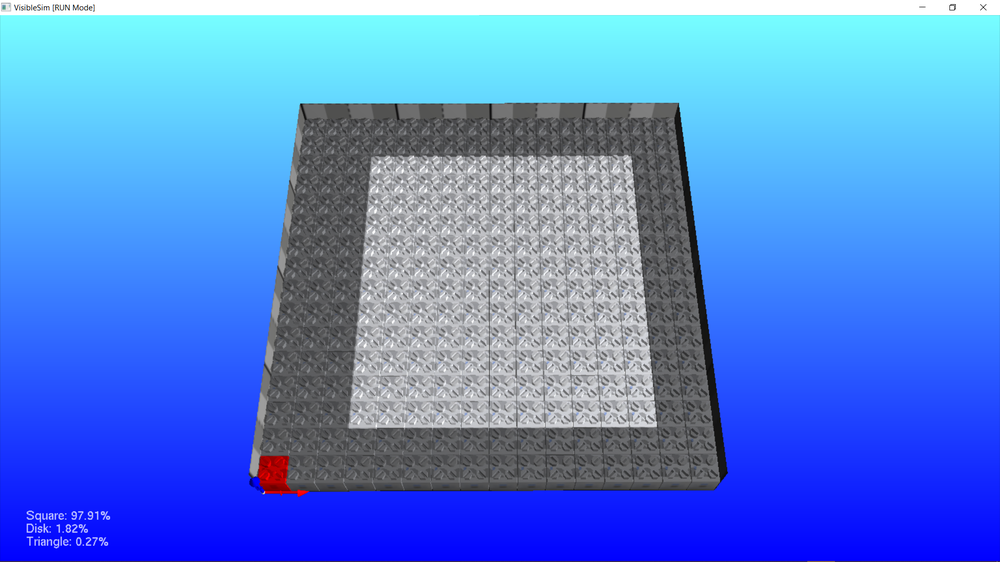
\includegraphics[width=0.23\textwidth]{figures/AI4PM/2D/ann2d_square.png}\hfill
    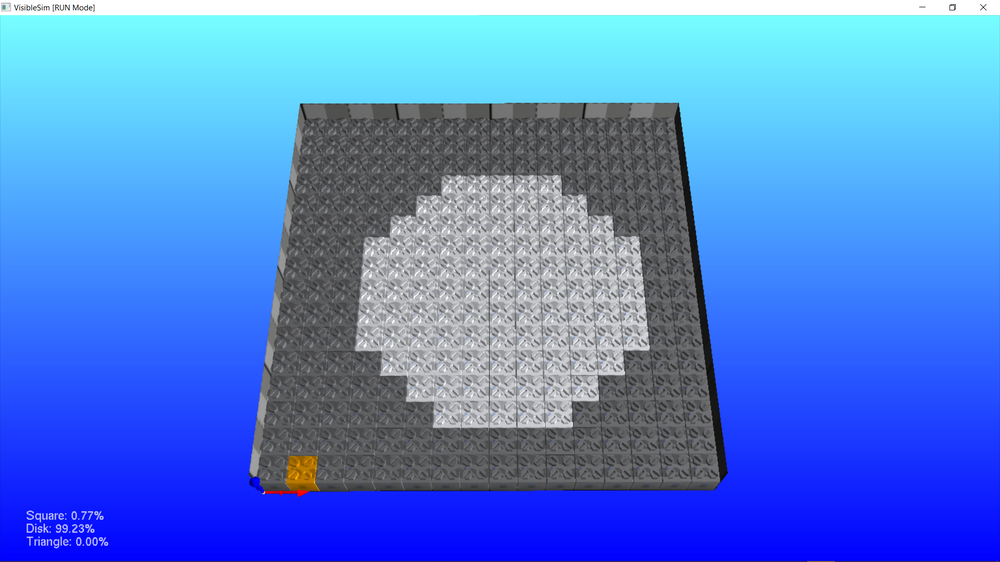
\includegraphics[width=0.23\textwidth]{figures/AI4PM/2D/ann2d_disk.png}\hfill
    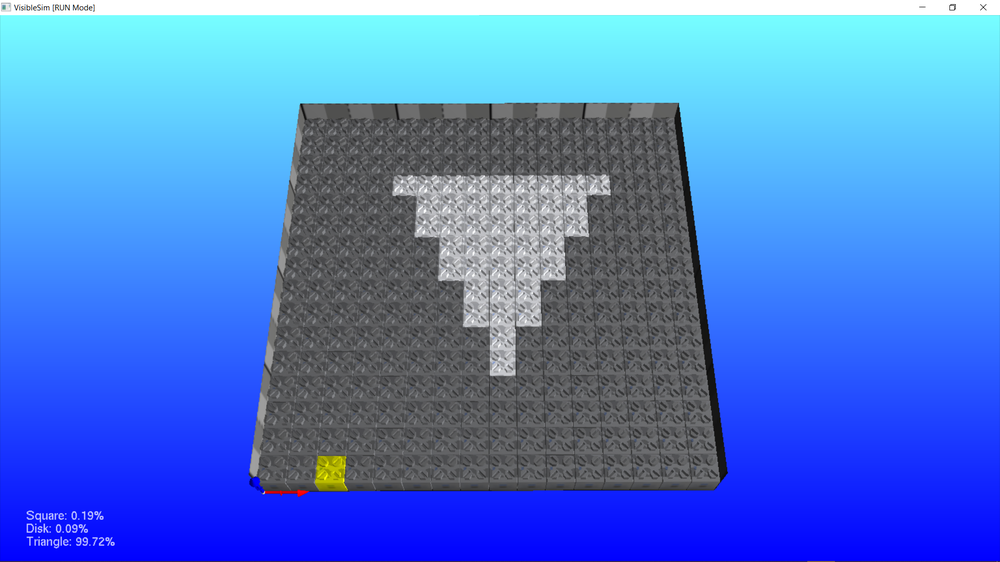
\includegraphics[width=0.23\textwidth]{figures/AI4PM/2D/ann2d_triangle.png}\hfill
    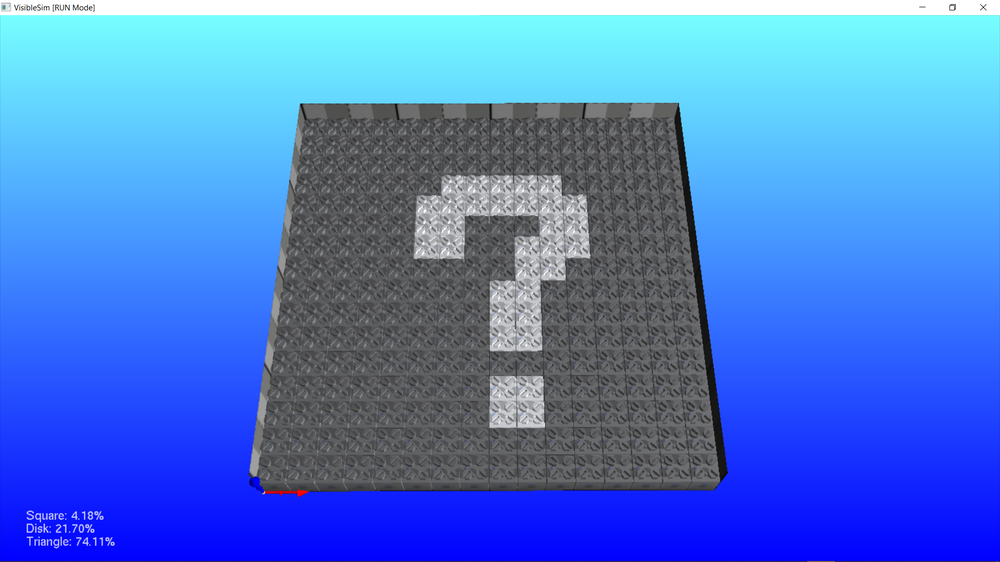
\includegraphics[width=0.23\textwidth]{figures/AI4PM/2D/ann2d_ambiguous.png}
    \caption{Stage 1 VisibleSim results. Left to right: Square, Disk, Triangle, and the ambiguous out-of-distribution test shape.}
    \label{fig:stage1}
\end{figure}

\subsection*{Discussion}

The quantized reproduction performs essentially identically to Piranda et al.'s reported results: all three trained classes are classified with confidence above 97\%, confirming that int8 weight quantization introduces no meaningful accuracy loss at this scale. The message count is identical (79,046) across all four runs regardless of the shape being classified, since the flat, fully-connected architecture always propagates every input unit's contribution to every hidden unit, irrespective of how much of the grid is actually occupied. The fourth run, on the deliberately unlabeled ambiguous shape, produces a plausible, non-degenerate probability split (74.11\% Triangle, 21.70\% Disk, 4.18\% Square) rather than a spuriously confident wrong answer, which is a reasonable behavior for a shape that does not resemble any trained class closely. This stage's fixed, shape-independent message count of 79,046 is the baseline against which Stage~2's scaling problem, described next, is measured.

\section{Stage 2: 3D-Extended ANN}
\label{sec:stage2}

\subsection*{Motivation and Design}

Stage~2 tested the most direct possible extension of Piranda et al.'s architecture to 3D: keep the same flat, fully-connected design, but replace the 16$\times$16 2D input grid with a 16$\times$16$\times$16 3D occupancy grid (4096 input units), and retrain against three 3D shape classes, which are the Cube, Sphere, and Cylinder, in place of the original Square, Disk, and Triangle. This stage was deliberately a naive extension rather than a redesign, precisely in order to measure, under otherwise matched conditions, what happens to a flat architecture's message count and accuracy once it is asked to classify genuinely volumetric shapes.

\subsection*{Implementation}

The training scripts for this stage are \texttt{applicationsSrc/AI4PM3D/tinyml\_ai4pm\_3d\_v0.py} through \texttt{v4.py} and \texttt{tinyml\_ai4pm\_3d.py}, and the corresponding firmware is implemented in \texttt{applicationsSrc/AI4PM3D/AI4PM3D.cpp}, \texttt{AI4PMCode3D.cpp}, and \texttt{AI4PMCode3D.hpp}. The trained weights are exported to \texttt{neuralNetworkData\_3d.h}. The five successive script versions (\texttt{v0} through \texttt{v4}) reflect several rounds of attempting to improve this flat architecture's accuracy directly, through changes to the training data generator, the hidden-layer width, and the training schedule, before the message-count results reported below made it clear that no amount of retraining could address the underlying architectural scaling problem, and that a different architectural family, rather than a better-trained instance of the same one, was required.

\subsection*{Results}

Table~\ref{tab:stage2-results} reports three VisibleSim runs, one per shape class. Figure~\ref{fig:stage2} shows the corresponding visualizations.

\begin{table}[H]
    \centering
    \caption{Stage 2 (3D-extended flat ANN) VisibleSim results.}
    \label{tab:stage2-results}
    \begin{tabular}{lcccccc}
        \toprule
        Config & Predicted & Cube & Sphere & Cylinder & Robots & Messages \\
        \midrule
        config\_sphere3d.xml   & Sphere (weak)   & 2.43\%  & 74.99\% & 22.58\% & 804 & 4,997,916 \\
        config\_cube3d.xml     & Cube (weak)     & 59.37\% & 0.23\%  & 40.39\% & 704 & 2,155,142 \\
        config\_cylinder3d.xml & Cylinder (strong) & 0.60\% & 0.20\%  & 99.21\% & 828 & 2,827,654 \\
        \bottomrule
    \end{tabular}
\end{table}

\begin{figure}[H]
    \centering
    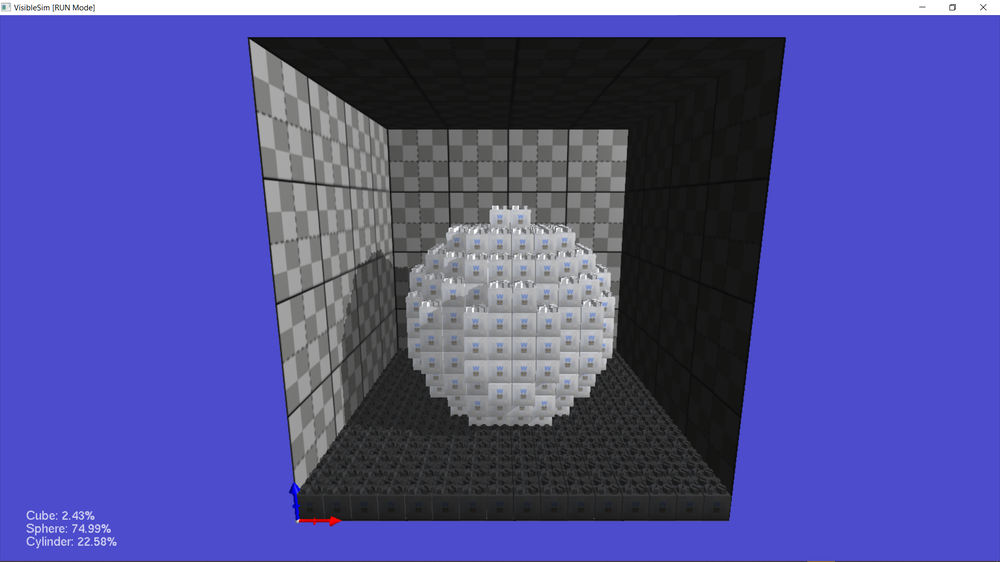
\includegraphics[width=0.31\textwidth]{figures/AI4PM/3D/ann3d_sphere.png}\hfill
    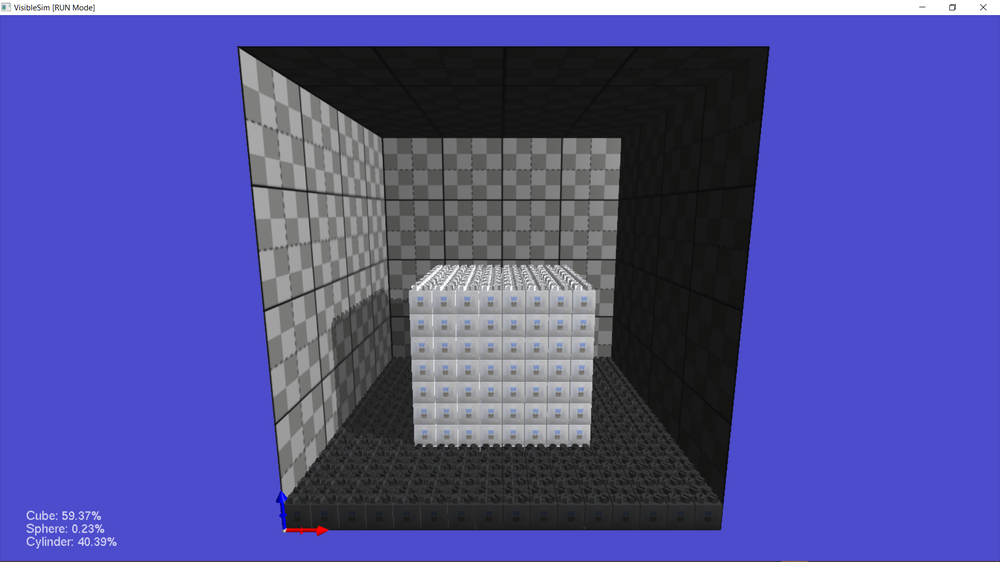
\includegraphics[width=0.31\textwidth]{figures/AI4PM/3D/ann3d_cube.png}\hfill
    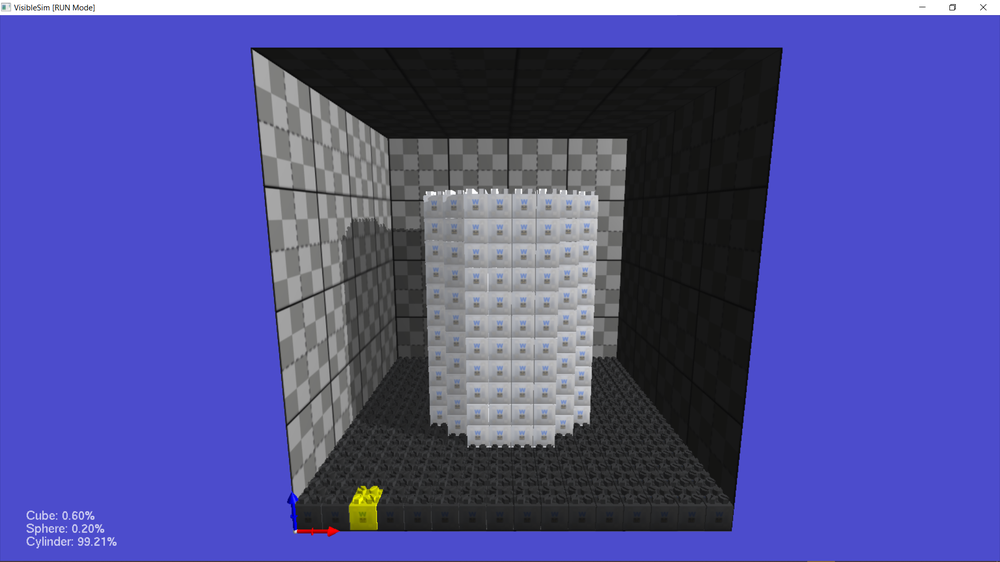
\includegraphics[width=0.31\textwidth]{figures/AI4PM/3D/ann3d_cylinder.png}
    \caption{Stage 2 VisibleSim results. Left to right: Sphere, Cube, Cylinder.}
    \label{fig:stage2}
\end{figure}

\subsection*{Discussion}

The results of this stage make the scaling problem anticipated in Section~1.2 directly measurable. The message count, which was a constant 79,046 in Stage~1, now ranges from roughly 2.15 million to nearly 5 million, an increase of two to three orders of magnitude for a model classifying the same number of shape classes (three). This growth is a direct consequence of the flat architecture's fully-connected input layer: a 4096-unit 3D input layer has sixteen times as many units as the 256-unit 2D input layer of Stage~1, and since every input unit's activation must still be message-passed to every hidden unit exactly as before, the communication cost scales at least linearly with input size, compounded further by the additional aggregation overhead of a physically larger, more deeply-connected 3D lattice. Confidence also degrades markedly on two of the three classes: Sphere is correctly identified but with only 74.99\% confidence, and Cube is correctly identified with only 59.37\% confidence, a substantial drop from Stage~1's consistently 97\%+ figures. Only Cylinder, whose extruded, axis-aligned silhouette is closest in spirit to the flat, per-slice occupancy pattern the network was trained on, retains high (99.21\%) confidence. Taken together, these results confirmed that a flat, fully-connected architecture is not a viable path toward richer 3D shape recognition on BlinkyBlocks, and motivated the shift to a convolutional, locally-computed architecture explored starting at Stage~3.

It is worth being precise about why this message-count explosion occurs, since the same underlying mechanism reappears, in a much smaller form, at every later stage whenever a design choice reintroduces even partial full connectivity. In Piranda et al.'s original architecture, and in this stage's naive 3D extension of it, every one of the network's 256 (or, here, 4096) input units must have its activation delivered, via message passing, to every one of the network's 64 hidden units, because the hidden layer's weighted sum genuinely depends on every input unit's value. There is no way to compute a fully-connected layer's output using only local, face-neighbor information, because by definition a fully-connected layer's output at any one unit depends on the entire input, not just a small neighborhood of it. A convolutional layer, by contrast, computes its output at any one spatial position from only a small, fixed-size neighborhood of the input around that position, which is precisely the property that lets Stage~3 onward implement each convolutional layer using only face-neighbor message exchange, with no fully-connected fan-out at all. This stage's results are, in effect, an empirical demonstration of exactly the architectural mismatch that motivated Dobreva et al.'s convolutional approach to distributed robot control (Section~2.3), now measured directly in message counts on the same platform and task family this thesis targets.

\section{Stage 3: 2D CNN}
\label{sec:stage3}

\subsection*{Motivation and Design}

Stage~3 replaced the flat, fully connected layers of Stages~1 and~2 with a convolutional architecture, computed locally by each block and propagated to face-neighbors via message passing, as motivated by Dobreva et al.'s demonstration that convolution composes naturally with a lattice system's native face-adjacent communication topology (Section~2.3). To isolate the effect of this architectural change from the effect of moving to 3D, Stage~3 was deliberately re-tested on Piranda et al.'s original 2D, 16$\times$16-grid, 256-block configuration, the same physical setup as Stage~1, so that the resulting message counts could be compared directly and fairly against Stage~1's flat-ANN baseline.

\subsection*{Implementation}

The training script for this stage is \texttt{applicationsSrc/AI4PM/tinyml\_ai4pm\_cnn.py}, and the firmware is implemented in (applicationsSrc/AI4PM/AI4PM\_CNN.cpp), \texttt{AI4PMCode\_CNN.cpp}, and \texttt{AI4PMCode\_CNN.hpp}. The firmware defines dedicated message types for the convolutional pipeline (\texttt{PixelMsgData} for the raw occupancy input, \texttt{Conv1MsgData} for first-layer feature exchange, and message identifiers \texttt{PIXEL\_MSG\_ID}, \texttt{CONV1\_MSG\_ID}, \texttt{CONV2\_MSG\_ID}, and \texttt{SOFTMAX\_MSG\_ID} for the successive pipeline phases), each block computing its local convolution from its own occupancy value and those of its immediate lattice neighbors. Notably, this stage's training data generator already relabels the three shape classes as Cube, Cylinder, and Triangle (rather than Piranda et al.'s original Square, Disk, and Triangle), even though the underlying test configurations remain flat 2D CSG cross-sections: a square-shaped 2D region is now labeled ``Cube'' and a disk-shaped 2D region is labeled ``Cylinder,'' anticipating the 3D shape vocabulary that would be adopted from Stage~2 onward.

\subsection*{Results}

Table~\ref{tab:stage3-results} reports four VisibleSim runs: the three trained classes plus one additional out-of-distribution ``question mark'' CSG shape used to test the model's behavior on an unfamiliar input. Figure~\ref{fig:stage3} shows the corresponding visualizations.

\begin{table}[H]
    \centering
    \caption{Stage 3 (2D CNN) VisibleSim results, 256 robots throughout.}
    \label{tab:stage3-results}
    \begin{tabular}{lcccccc}
        \toprule
        Config & Predicted & Cube & Cylinder & Triangle & Messages \\
        \midrule
        config\_cube\_csg.xml     & Cube     & 99.976\% & 0.0234\% & 0.0002\% & 1,161 \\
        config\_cylinder\_csg.xml & Cylinder & 0.0287\% & 99.930\% & 0.0417\% & 1,161 \\
        config\_triangle\_csg.xml & Triangle & 0.0045\% & 0.1149\% & 99.881\% & 1,161 \\
        config\_question\_csg.xml & (ambiguous) & 41.40\% & 22.63\% & 35.96\% & 1,161 \\
        \bottomrule
    \end{tabular}
\end{table}

\begin{figure}[H]
    \centering
    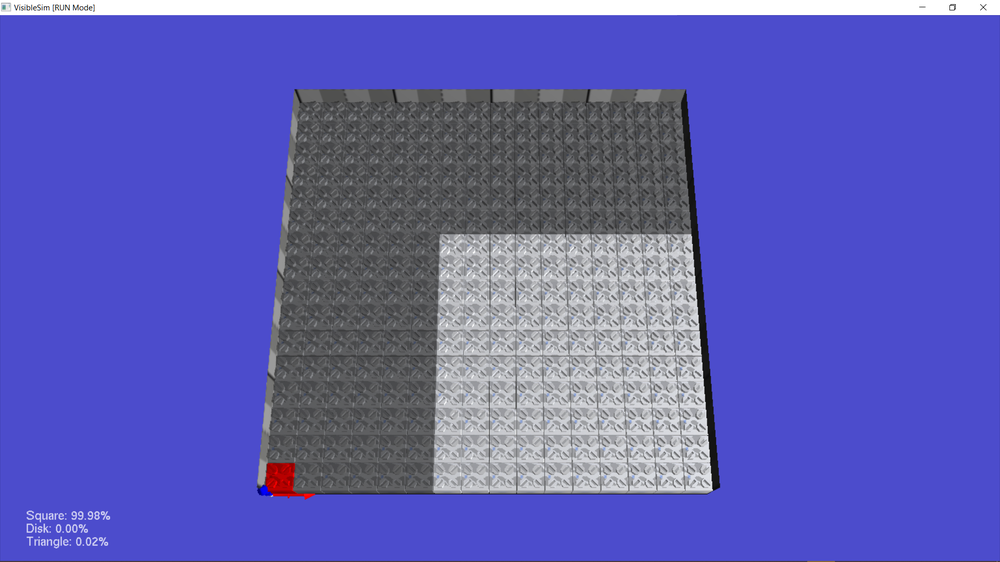
\includegraphics[width=0.23\textwidth]{figures/AI4PM-CNN/AI4PM_CNN/cnn2d_cube.png}\hfill
    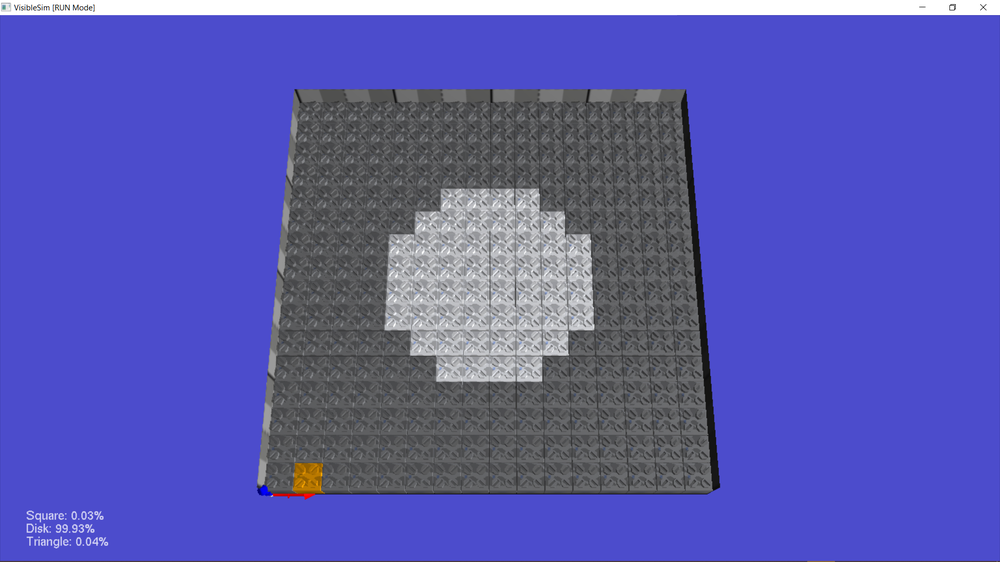
\includegraphics[width=0.23\textwidth]{figures/AI4PM-CNN/AI4PM_CNN/cnn2d_cylinder.png}\hfill
    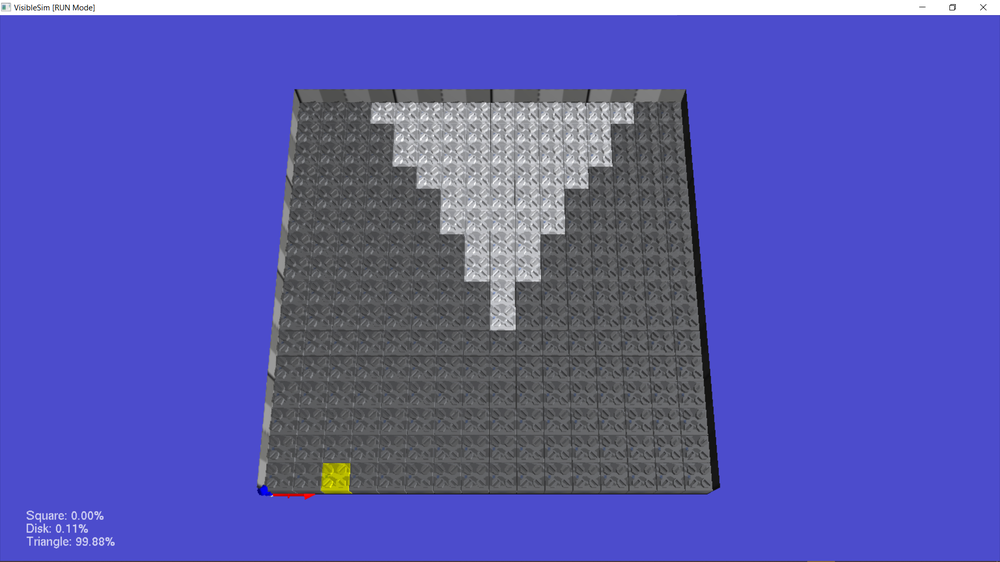
\includegraphics[width=0.23\textwidth]{figures/AI4PM-CNN/AI4PM_CNN/cnn2d_triangle.png}\hfill
    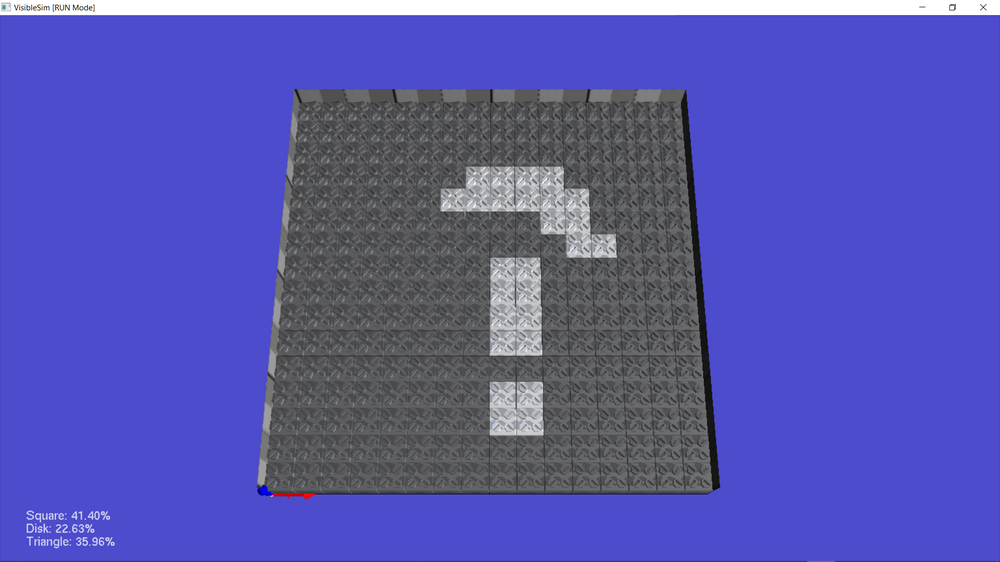
\includegraphics[width=0.23\textwidth]{figures/AI4PM-CNN/AI4PM_CNN/cnn2d_question.png}
    \caption{Stage 3 VisibleSim results. Left to right: Cube (square silhouette), Cylinder (disk silhouette), Triangle, and the out-of-distribution question-mark shape.}
    \label{fig:stage3}
\end{figure}

\subsection*{Discussion}

The efficiency gain from switching to a convolutional, locally computed architecture is immediate and large: on the exact same 256-block, 16$\times$16 configuration as Stage~1, the message count drops from 79,046 to just 1,161, roughly a 68x reduction, while classification confidence on all three trained classes remains above 99.8\%, matching or exceeding Stage~1's flat-ANN accuracy. This confirms directly, under matched conditions, that convolution's local, face-adjacent computation pattern is dramatically cheaper to message-pass than a fully-connected layer's all-to-all connectivity, without sacrificing accuracy. The out-of-distribution ``question mark'' test further shows the model behaving sensibly under genuine ambiguity: rather than confidently misclassifying an unfamiliar shape, it produces a comparatively flat probability distribution (41.40\% / 22.63\% / 35.96\%), evidence that the learned convolutional features are meaningfully tied to the trained shapes' actual geometry rather than to spurious grid-position artifacts. These results validated convolution with local message passing as the right general direction, and the next stage's task was to extend this same efficient design from 2D to genuinely volumetric 3D shapes.

It is also worth noting what this stage's convolutional pipeline still shares with Piranda et al.'s original design, since the two are easy to conflate given how different their message-count results are. Both architectures still rely on a small set of dedicated aggregation agents (Piranda et al.'s Super Node and Divider agents, and this stage's equivalent classification-aggregation logic) to combine the many parallel local outputs into a single structure-wide decision; the reduction from ``many local feature vectors'' to ``one classification result'' is not itself a convolution, and still requires some form of tree-based or otherwise structured aggregation across the whole occupied lattice. What changed between Stage~1 and this stage is not whether aggregation happens, but how much work each individual block does, and how far each unit of information has to travel, before that aggregation step: a fully-connected layer requires every input to reach every hidden unit before aggregation can even begin, whereas a convolutional layer's output at each block already summarizes only that block's own local neighborhood, so the aggregation step that follows has much less redundant information to combine.

\section{Stage 4: 3D CNN via Height-Map Projection}
\label{sec:stage4}

\subsection*{Motivation and Design}

Stage~4 extended Stage~3's 2D CNN to 3D shapes. Rather than building a genuinely 3D convolutional pipeline from scratch, this stage reused the existing, already-validated 2D CNN architecture unchanged, and instead transformed the 3D input into a form that architecture could consume: every block at the base layer of the lattice (height $z=0$) queries the column of blocks directly above it and computes a normalized height value, effectively how many blocks are stacked at that $(x,y)$ position, producing a 16$\times$16 ``height-map'' image that is then fed into the same 2D CNN pipeline used at Stage~3. Only the base-layer blocks perform this height-map projection; every other block in the structure plays no role in the classification computation at all.

\subsection*{Implementation}

The firmware for this stage is implemented in \texttt{applicationsSrc/AI4PM3D/AI4PM\_CNN\_3D.cpp}, \texttt{AI4PMCode\_CNN\_3D.cpp}, and \texttt{AI4PMCode\_CNN\_3D.hpp}, with the corresponding training script in \texttt{applicationsSrc/AI4PM3D/tinyml\_3d\_heightmap.py}. Choosing this height-map projection as an interim design, rather than jumping directly to a fully embedded 3D convolution, was a deliberate scoping decision: it made it possible to reuse Stage~3's already-trained, already-validated 2D CNN weights and message-passing logic essentially unchanged, isolating the height-map projection step itself as the only new piece of firmware that needed to be designed, implemented, and debugged before this stage's results could be trusted.

\subsection*{Results}

Table~\ref{tab:stage4-results} reports three VisibleSim runs, one per shape class, with the robot (block) count now varying by shape since the total number of blocks in a 3D solid depends on its volume, unlike the fixed 256-block 2D grid of Stages~1 and~3. Figure~\ref{fig:stage4} shows the corresponding visualizations, including the colored height-map pattern visible on the base layer beneath each 3D shape.

\begin{table}[H]
    \centering
    \caption{Stage 4 (height-map 3D CNN) VisibleSim results.}
    \label{tab:stage4-results}
    \begin{tabular}{lcccccc}
        \toprule
        Config & Predicted & Cube & Sphere & Cylinder & Robots & Messages \\
        \midrule
        config\_cylinder\_csg.xml & Cylinder & 0.034\% & 0.491\%  & 99.475\% & 577 & 1,161 \\
        config\_sphere\_csg.xml   & Sphere   & 0.049\% & 96.895\% & 3.057\%  & 572 & 1,161 \\
        config\_cube\_csg.xml     & Cube     & 96.271\% & 3.121\% & 0.608\%  & 599 & 1,161 \\
        \bottomrule
    \end{tabular}
\end{table}

\begin{figure}[H]
    \centering
    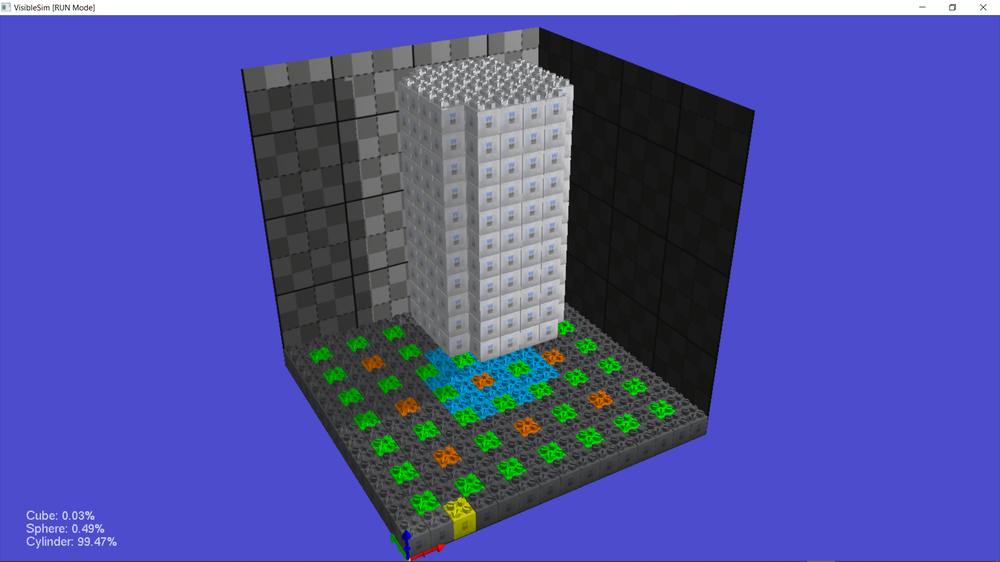
\includegraphics[width=0.31\textwidth]{figures/AI4PM-CNN/AI4PM_CNN_3D/cnn3d_hm_cylinder.png}\hfill
    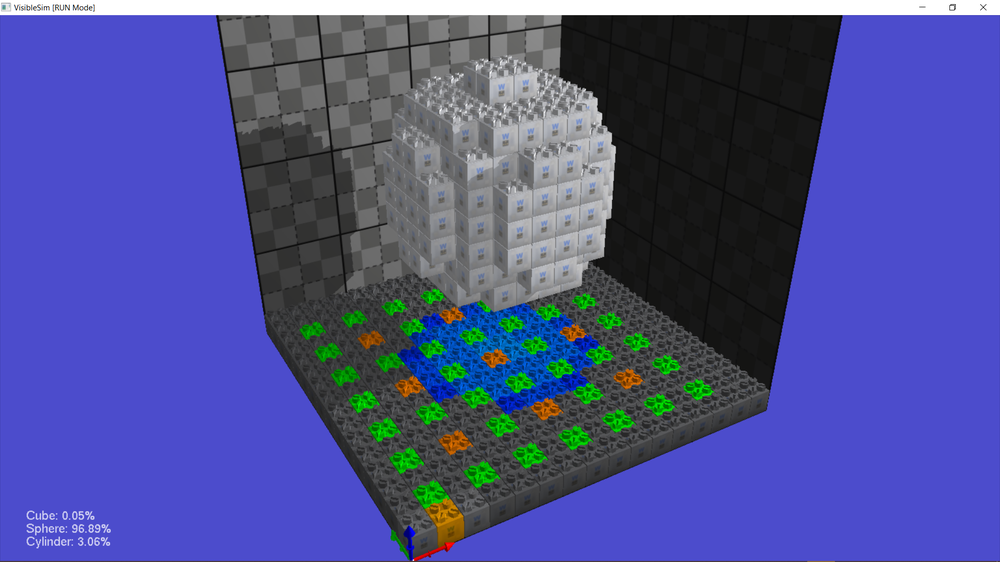
\includegraphics[width=0.31\textwidth]{figures/AI4PM-CNN/AI4PM_CNN_3D/cnn3d_hm_sphere.png}\hfill
    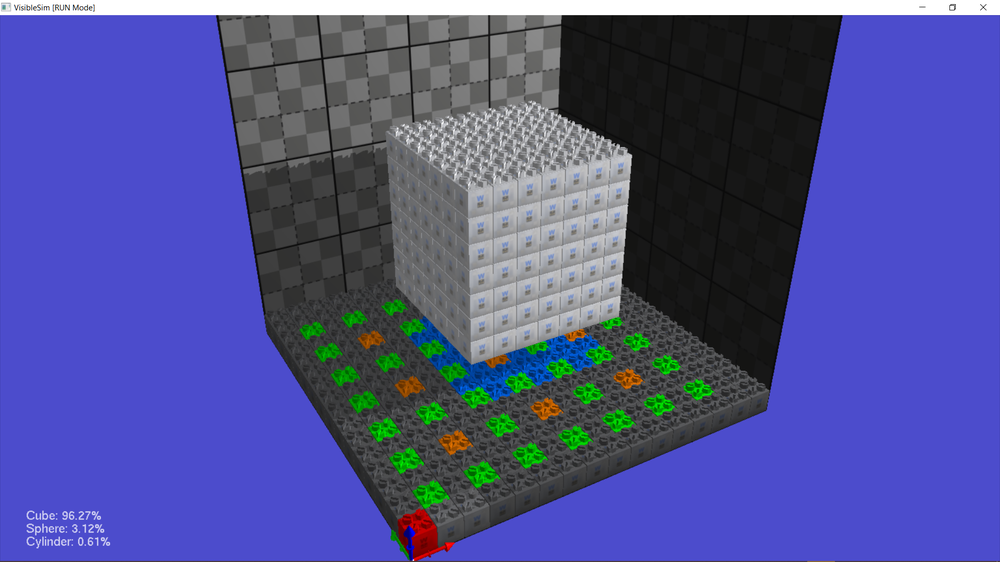
\includegraphics[width=0.31\textwidth]{figures/AI4PM-CNN/AI4PM_CNN_3D/cnn3d_hm_cube.png}
    \caption{Stage 4 VisibleSim results. Left to right: Cylinder, Sphere, Cube. The colored base-layer pattern beneath each shape is the height-map projection consumed by the 2D CNN.}
    \label{fig:stage4}
\end{figure}

\subsection*{Discussion}

This stage confirms that Stage~3's efficiency gain carries over to 3D shapes: the message count remains fixed at exactly 1,161, identical to Stage~3, since the underlying computation is still the same 2D CNN operating on a 16$\times$16 height-map, regardless of how many blocks actually make up the 3D structure above it. Accuracy remains strong across all three classes (96.27\% to 99.48\%). However, this stage's design carries a structural limitation that is at least as important as its results: only the fixed set of base-layer ($z=0$) blocks perform the height-map projection and subsequent convolution; every other block in the structure is, from the classification algorithm's point of view, inert. This means the architecture implicitly depends on a hardcoded notion of ``which blocks are allowed to participate,'' tied to a specific physical orientation of the structure relative to a base plane: a shape rotated so that its silhouette no longer projects cleanly onto that base plane would not be correctly summarized by the height-map, and a block that happened not to be part of the $z=0$ layer in a given assembly could never contribute to or benefit from the classification result. This hardcoded-position dependency, rather than an accuracy or efficiency shortfall, is what motivated Stage~5's redesign.

The height-map approach can be understood as trading one form of centralization for another. Stages~1 and~2's flat ANNs were centralized in the sense that every input had to reach every hidden unit; this stage is centralized in a different, more subtle sense, in that a small, fixed, physically-located subset of blocks (the $z=0$ base layer) is implicitly treated as more important than the rest of the structure, even though the message-passing pattern used to reach that conclusion is itself perfectly local and face-neighbor-based. This is precisely the kind of hardcoded assumption that a genuine Programmable Matter deployment cannot tolerate: a real assembled structure has no guarantee that a ``base layer'' aligned with the designer's assumed coordinate frame will exist at all, particularly once the structure is capable of self-reconfiguring or being assembled in an arbitrary orientation. Recognizing this was the key conceptual step that led directly to Stage~5's design, which asks a more demanding but more principled question: can every block, with no exceptions and no privileged roles, contribute equally to the classification result?

\section{Stage 5: Embedded 3D CNN}
\label{sec:stage5}

\subsection*{Motivation and Design}

Stage~5 removed the height-map hack entirely. Instead of a privileged base layer performing a projection that every other block depends on, every block in the assembled structure now runs the same local convolution over its own immediate face-neighborhood, with no block assigned any special, hardcoded role. Concretely, each block first computes a local feature vector directly from its own occupancy state (\texttt{computeConv1}, requiring no messages), then exchanges that feature vector with its face-connected neighbors and computes a second local feature vector from the combination (\texttt{computeConv2}, requiring one round of face-neighbor message passing). A spanning tree, rooted dynamically rather than at any fixed physical position, is then constructed across the occupied blocks to aggregate every block's final feature vector into a single classification decision, which is then broadcast back out to the whole structure, the same general aggregation pattern used by Piranda et al.'s Super Node and Divider agents (Section~2.2), but now applied to convolutional features computed at every block rather than to a flat network's fully-connected activations.

\subsection*{Implementation}

The firmware for this stage is implemented in \texttt{applicationsSrc/AI4PM3D/AI4PM\_Embedded3D.cpp}, \texttt{AI4PMCode\_Embedded3D.cpp}, and \texttt{AI4PMCode\_Embedded3D.hpp}, with trained weights exported to \texttt{neuralNetworkData\_embedded3d.h}. This stage's firmware also introduces explicit phase-by-phase diagnostic logging (\texttt{PHASE 3: Spanning Tree (BFS) Construction}, \texttt{PHASE 4: Global Feature Aggregation (Pooling)}, \texttt{PHASE 5: Classification Verdict \& Global Broadcast}), a logging convention that is preserved and extended in Stage~6's firmware.

\subsection*{Results}

Table~\ref{tab:stage5-results} reports four VisibleSim runs across the three trained classes, including one additional run repeating the Cylinder configuration after a 90\textdegree{} rotation about the Y axis, specifically to test whether the removal of the height-map's implicit orientation dependency (Stage~4's limitation) had actually been resolved. Figure~\ref{fig:stage5} shows the corresponding visualizations.

\begin{table}[H]
    \centering
    \caption{Stage 5 (Embedded 3D CNN) VisibleSim results.}
    \label{tab:stage5-results}
    \begin{tabular}{lccccc}
        \toprule
        Config & Predicted (confidence) & Blocks aggregated & Messages \\
        \midrule
        config\_sphere\_csg.xml                    & Sphere (100.0\%)   & 316 & 4,074 \\
        config\_cube\_csg.xml                      & Cube (93.4\%)      & 343 & 4,608 \\
        config\_cylinder\_csg.xml                  & Cylinder (100.0\%) & 416 & 5,530 \\
        config\_cylinder\_csg.xml (rotated 90\textdegree{} Y) & Cylinder (100.0\%) & 312 & 4,046 \\
        \bottomrule
    \end{tabular}
\end{table}

\begin{figure}[H]
    \centering
    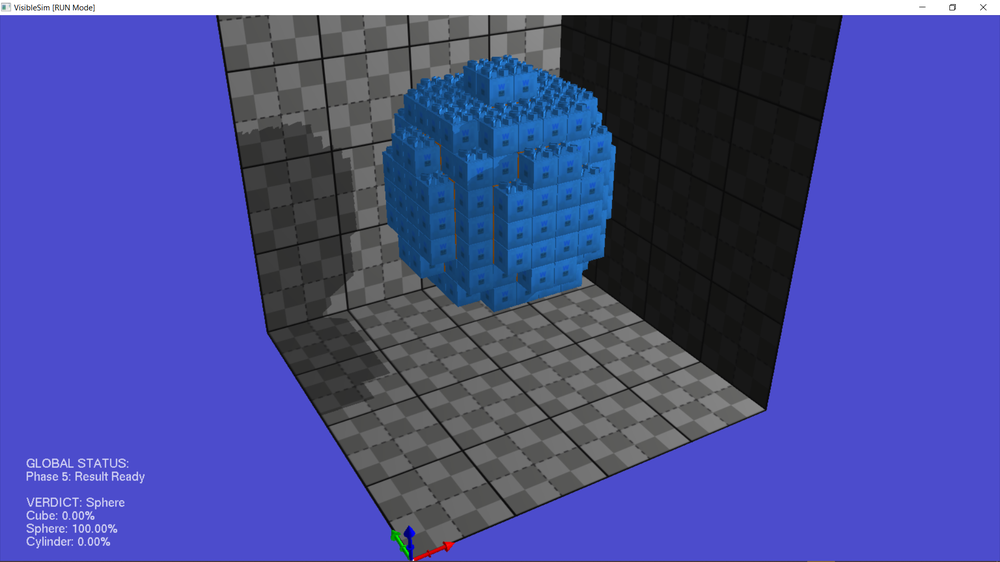
\includegraphics[width=0.23\textwidth]{figures/AI4PM-CNN/AI4PM-Embedded/embedded_sphere.png}\hfill
    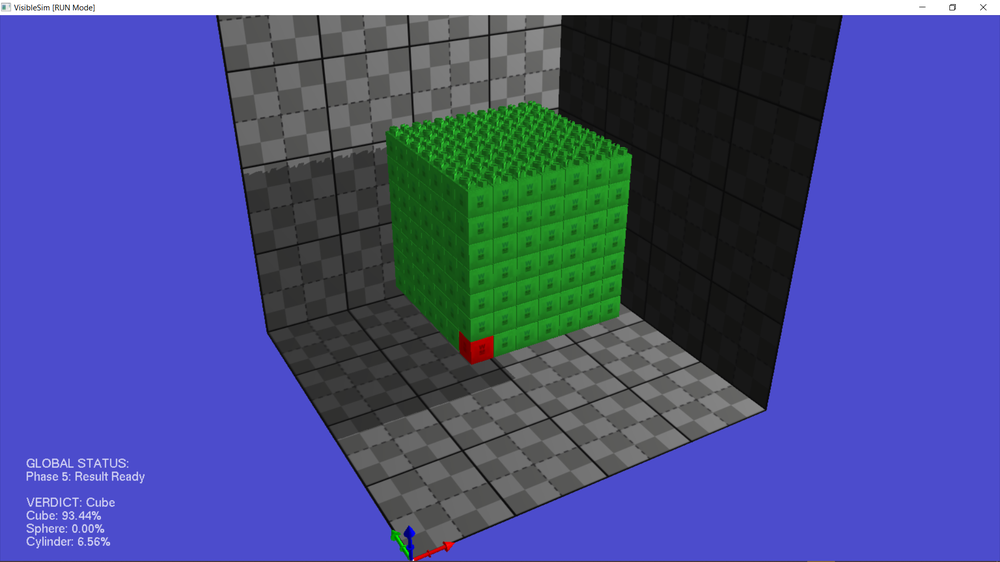
\includegraphics[width=0.23\textwidth]{figures/AI4PM-CNN/AI4PM-Embedded/embedded_cube.png}\hfill
    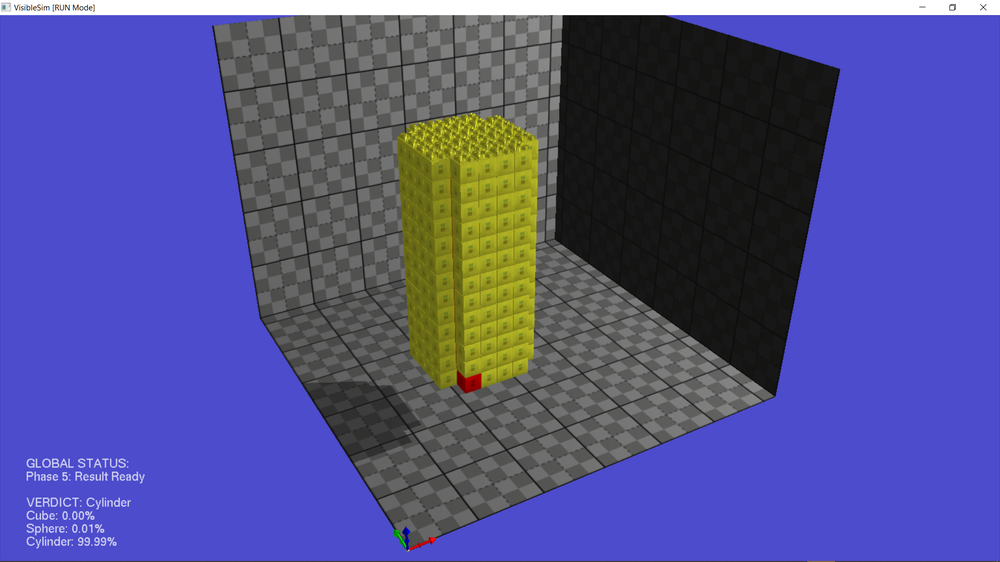
\includegraphics[width=0.23\textwidth]{figures/AI4PM-CNN/AI4PM-Embedded/embedded_cylinder.png}\hfill
    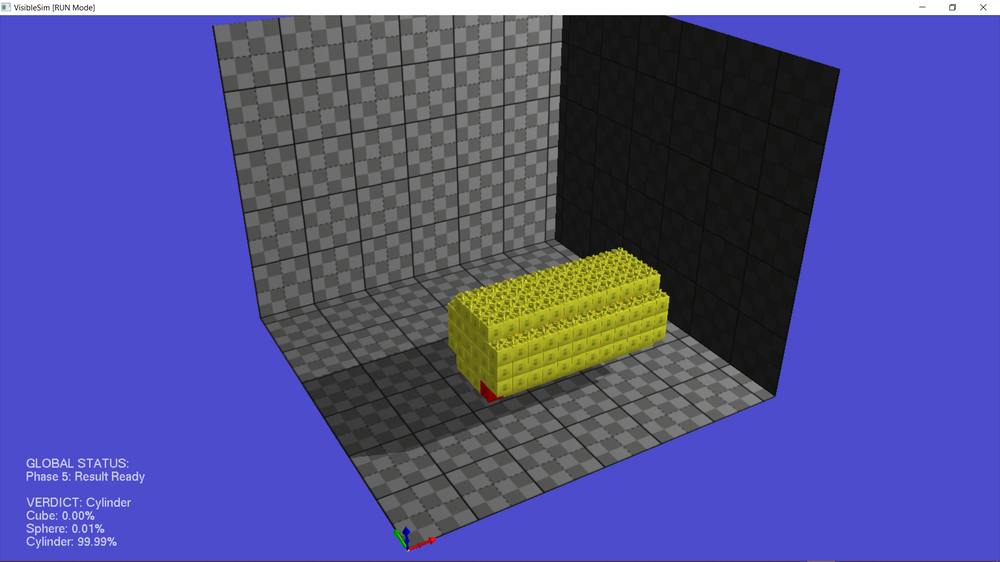
\includegraphics[width=0.23\textwidth]{figures/AI4PM-CNN/AI4PM-Embedded/embedded_cylinder_rotated.png}
    \caption{Stage 5 VisibleSim results. Left to right: Sphere, Cube, Cylinder (upright), and the same Cylinder rotated 90\textdegree{} about the Y axis (lying on its side).}
    \label{fig:stage5}
\end{figure}

\subsection*{Discussion}

Two results from this stage are particularly significant. First, the message count is no longer a fixed, shape-independent constant (as it was at 1,161 for both Stages~3 and~4): it now scales with the actual number of blocks aggregated (316 to 416 blocks, 4,046 to 5,530 messages), confirming that communication cost in this architecture is genuinely proportional to the physical size of the structure being classified, rather than to a fixed 2D projection resolution. Second, the rotated-Cylinder test directly confirms that Stage~4's hardcoded-orientation limitation has been resolved: the same physical shape, rotated 90\textdegree{} so that its long axis is no longer aligned with the lattice's vertical axis, is still classified correctly with 100.0\% confidence and a comparable message count (4,046 versus 5,530 for the upright case). This stage's remaining limitations, motivating the final Stage~6, are its shallow depth (only two convolutional phases) and its restriction to the same three shape classes used throughout Stages~2, 4, and 5.

Beyond these two specific limitations, this stage is also the point in this thesis's progression where the general architectural pattern that Stage~6 would later extend was fully established: local computation with no messages (Conv1), one round of face-neighbor message exchange and local combination (Conv2), and a dynamically-rooted spanning-tree aggregation feeding a small classification head. Every one of these three components generalizes cleanly to additional convolutional phases (simply repeating the message-exchange-and-combine step of Conv2 with a new set of weights, as Stage~6's Conv3 does) and to additional output classes (simply widening the final classification head's output layer), without requiring any change to the underlying communication pattern. This generality is what made Stage~6 achievable as an extension of this stage's design, rather than requiring another full architectural redesign.

\section{Stage 6: Deep Embedded 3D CNN and TinyML Int8 Quantization}
\label{sec:stage6}

Stage~6 is both the final architecture developed during this internship and the one ultimately deployed to real BlinkyBlocks hardware. It extends Stage~5's embedded, no-hardcoded-position design with one additional convolutional phase (three convolutional phases in total, rather than two), a wider shape vocabulary (six classes, which are Cube, Sphere, Cylinder, Chair, Bridge, and Humanoid, rather than three), and, critically, TinyML int8 weight quantization applied to make the resulting deeper model deployable within BlinkyBlocks' flash memory budget. This section presents this final architecture in full technical detail, since it is the direct subject of the conference paper produced from this internship's work.

\subsection{Shape Representation}

Each module is placed in one cell of a 3D lattice, and the structure that is formed is a binary occupancy volume, where a cell is 1 if a BlinkyBlock is present at that position, and 0 otherwise. Each module then only ever needs to consider the local neighborhood of occupancy around its own position, rather than the shape as a whole, which is what makes a convolutional approach a natural fit: a 3D convolution is by definition a local operation over a neighborhood, and that neighborhood can be made to correspond exactly with the face-connections a BlinkyBlock physically has to its neighbors.

\subsection{Network Architecture}

The whole pipeline is illustrated in Figure~\ref{fig:architecture}, which is divided into five phases performed sequentially by every module. The Conv1 operator is computed directly by each block over its own $3\times3\times3$ occupancy neighborhood, with no messages required. The second and third phases (Conv2, Conv3) are message-passed convolutions: each block exchanges its current $K$-dimensional feature vector with its 6 face-connected neighbors, concatenates the 7 vectors, and passes the result through a dense layer with a residual connection, mirroring a convolution restricted to face-adjacent cells (diagonally adjacent neighbors are not reachable in a single message hop). Each stage adds one more hop of face-neighbor context to the effective receptive field; this is the one additional convolutional phase, relative to Stage~5's two-phase design, that gives this architecture its name. Phase 4 performs masked global average pooling, distributed along a spanning tree in the same fashion as the Super Node and Divider agents of Piranda et al.~\cite{piranda2024ai4pm}. In Phase 5, a two-layer fully connected head produces a 6-way softmax over the shape classes.

This architecture generalizes the agent roles of Piranda et al.~\cite{piranda2024ai4pm} (Input, Layer, Output) into this thesis's Conv1, message-passed Conv2/Conv3, and pooling-and-classification stages, adding spatial locality and weight sharing so a single small set of weights generalizes across shapes of any size and position, the same property that resolved Stage~4's hardcoded-orientation limitation and Stage~5's fixed shape count, now extended one layer deeper.

\begin{figure}[H]
    \centering
    \resizebox{!}{7.2cm}{
    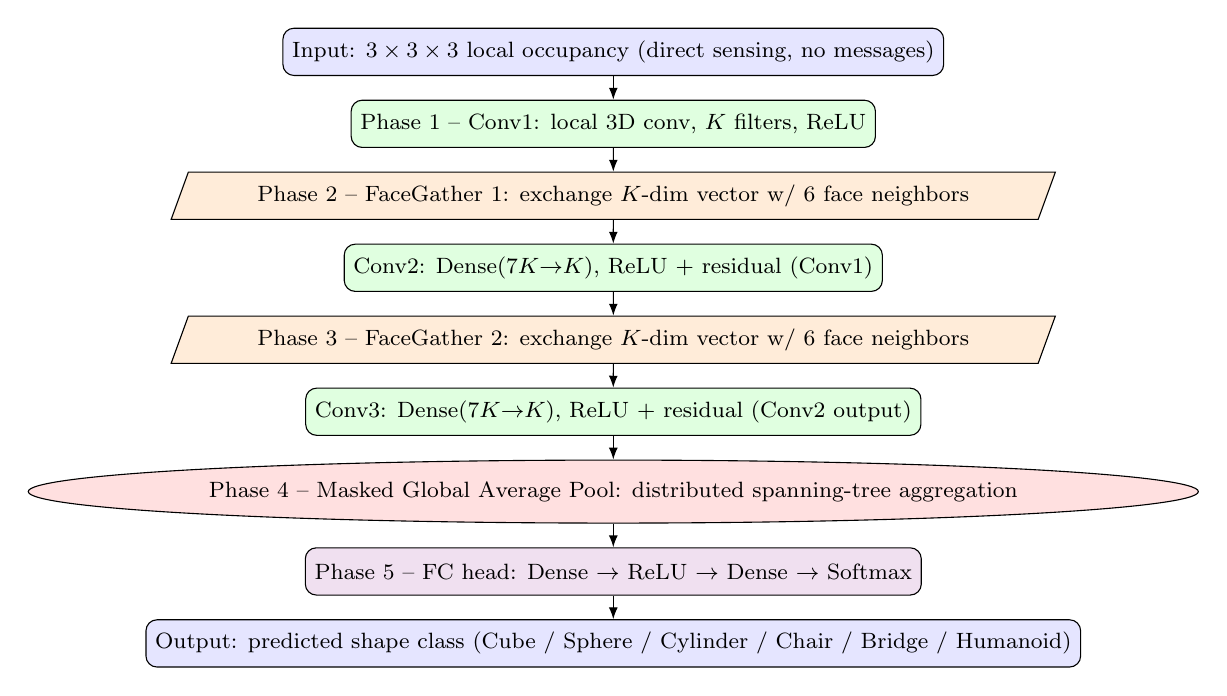
\begin{tikzpicture}[
        node distance=3mm,
        block/.style={rectangle, rounded corners, draw, fill=green!12, minimum width=6cm, minimum height=6mm, align=center, font=\footnotesize},
        msgblock/.style={trapezium, trapezium left angle=70, trapezium right angle=110, draw, fill=orange!15, minimum width=6cm, minimum height=6mm, align=center, font=\footnotesize},
        poolblock/.style={ellipse, draw, fill=red!12, minimum width=6cm, minimum height=8mm, align=center, font=\footnotesize},
        fcblock/.style={rectangle, rounded corners, draw, fill=violet!12, minimum width=6cm, minimum height=6mm, align=center, font=\footnotesize},
        ioblock/.style={rectangle, rounded corners, draw, fill=blue!10, minimum width=6cm, minimum height=6mm, align=center, font=\footnotesize},
        arr/.style={-{Latex[length=1.5mm]}}
    ]
        \node[ioblock] (input) {Input: $3\times3\times3$ local occupancy (direct sensing, no messages)};
        \node[block, below=of input] (conv1) {Phase 1 -- Conv1: local 3D conv, $K$ filters, ReLU};
        \node[msgblock, below=of conv1] (fg1) {Phase 2 -- FaceGather 1: exchange $K$-dim vector w/ 6 face neighbors};
        \node[block, below=of fg1] (conv2) {Conv2: Dense($7K{\to}K$), ReLU + residual (Conv1)};
        \node[msgblock, below=of conv2] (fg2) {Phase 3 -- FaceGather 2: exchange $K$-dim vector w/ 6 face neighbors};
        \node[block, below=of fg2] (conv3) {Conv3: Dense($7K{\to}K$), ReLU + residual (Conv2 output)};
        \node[poolblock, below=of conv3] (pool) {Phase 4 -- Masked Global Average Pool: distributed spanning-tree aggregation};
        \node[fcblock, below=of pool] (fc) {Phase 5 -- FC head: Dense $\to$ ReLU $\to$ Dense $\to$ Softmax};
        \node[ioblock, below=of fc] (output) {Output: predicted shape class (Cube / Sphere / Cylinder / Chair / Bridge / Humanoid)};

        \draw[arr] (input) -- (conv1);
        \draw[arr] (conv1) -- (fg1);
        \draw[arr] (fg1) -- (conv2);
        \draw[arr] (conv2) -- (fg2);
        \draw[arr] (fg2) -- (conv3);
        \draw[arr] (conv3) -- (pool);
        \draw[arr] (pool) -- (fc);
        \draw[arr] (fc) -- (output);
    \end{tikzpicture}
    }
    \caption{Stage 6 (Deep Embedded 3D CNN) distributed architecture}
    \label{fig:architecture}
\end{figure}

To summarize, the recognition process applies the following equations at each block. Let $V_{i,j,k}$ denote the block's local $3\times3\times3$ occupancy window ($i,j,k \in \{0,1,2\}$), and let $K$ be the number of feature channels per block.

\textbf{Phase 1 (Conv1, local, no messages):}
\begin{equation}
\text{Conv1}_f = \mathrm{ReLU}\left(b^{(1)}_f + \sum_{i,j,k=0}^{2} W^{(1)}_{f,i,j,k} \cdot V_{i,j,k}\right), \quad f = 1,\dots,K
\label{eq:conv1}
\end{equation}

\textbf{Phase 2 (Conv2, message-passed, 1 hop):} each block concatenates its own Conv1 output with the Conv1 outputs received from its 6 face neighbors into a $7K$-dimensional vector $X^{(2)}$, then applies:
\begin{equation}
\text{Conv2}_f = \mathrm{ReLU}\left(b^{(2)}_f + \sum_{i=1}^{7K} W^{(2)}_{f,i} \cdot X^{(2)}_i\right), \qquad H^{(2)}_f = \text{Conv2}_f + \text{Conv1}_f
\label{eq:conv2}
\end{equation}

\textbf{Phase 3 (Conv3, message-passed, 2nd hop):} identical in form to Phase 2, but built from $H^{(2)}$ instead of Conv1, giving a $7K$-dimensional $X^{(3)}$:
\begin{equation}
\text{Conv3}_f = \mathrm{ReLU}\left(b^{(3)}_f + \sum_{i=1}^{7K} W^{(3)}_{f,i} \cdot X^{(3)}_i\right), \qquad H^{(3)}_f = \text{Conv3}_f + H^{(2)}_f
\label{eq:conv3}
\end{equation}

\textbf{Phase 4 (distributed pooling):} the structure's total feature sum $S$ and occupied-block count $N$ are aggregated over a spanning tree rooted at one block, then averaged:
\begin{equation}
S = \sum_{\text{occupied blocks}} H^{(3)}, \qquad N = \sum_{\text{occupied blocks}} 1, \qquad A = S / N
\label{eq:pool}
\end{equation}

\textbf{Phase 5 (classification head, root only):}
\begin{equation}
Z = \mathrm{ReLU}(W^{(fc1)} A + b^{(fc1)}), \qquad P = \mathrm{Softmax}(W^{(fc2)} Z + b^{(fc2)})
\label{eq:fc}
\end{equation}

The distributed computation problem for Phases 2 and 3 is similar in nature to Piranda et al.~\cite{piranda2024ai4pm}: each receiving block must be aware once it has received a message from all of its face neighbors, since a message that will never arrive (e.g. from a boundary face with no neighbor) must not be waited on forever.

For this purpose we introduce three agents to map these phases onto BlinkyBlocks messages, shown in Algorithms~\ref{alg:phase1}--\ref{alg:phase45}.

\begin{algorithm}[H]
\caption{Phase 1: Local Feature Extraction (Conv1)}
\label{alg:phase1}
\begin{algorithmic}[1]
\Function{Startup}{}
    \State $V \gets \Call{QueryNeighborhood}{}$ \Comment{$3\times3\times3$ local occupancy scan}
    \For{$f \gets 1$ \textbf{to} $K$}
        \State $sum \gets b^{(1)}_f + \sum_{i,j,k} V_{i,j,k} \times W^{(1)}_{f,i,j,k}$
        \State $\text{Conv1}_f \gets \max(0, sum)$
    \EndFor
    \If{$ID = 1$}
        \State \Call{InitiateSpanningTree}{}
    \EndIf
    \State \Call{Broadcast}{Conv1} to face-neighbors
\EndFunction
\end{algorithmic}
\end{algorithm}

\begin{algorithm}[H]
\caption{Phases 2/3: Message-Passed Convolution (Conv2, Conv3)}
\label{alg:phase23}
\begin{algorithmic}[1]
\Function{HandleFeatureMsg}{msg}
    \State Save received feature vector from neighbor to memory
    \If{all face neighbors reported}
        \State $X \gets [H_{self}, H_{n_1}, \dots, H_{n_6}]$ \Comment{$7K$-dim concatenation}
        \For{$f \gets 1$ \textbf{to} $K$}
            \State $sum \gets b_f + \sum_i X_i \times W_{f,i}$
            \State $\text{Conv}_f \gets \max(0, sum) + H_{self,f}$ \Comment{residual add}
        \EndFor
        \State \Call{CheckReadyToAggregate}{}
    \EndIf
\EndFunction
\end{algorithmic}
\end{algorithm}

\begin{algorithm}[H]
\caption{Phases 4/5: Distributed Aggregation and Classification}
\label{alg:phase45}
\begin{algorithmic}[1]
\Function{CheckReadyToAggregate}{}
    \If{Conv3 done \textbf{and} in tree \textbf{and} all children done}
        \State $Sum \gets H^{(3)} + \sum \text{Sum}_{children}$
        \State $Count \gets 1 + \sum \text{Count}_{children}$
        \If{role is Root}
            \State \Call{Classify}{$Sum / Count$} \Comment{Eq.~\ref{eq:fc}}
        \Else
            \State \Call{SendAggregate}{$Sum, Count$} to parent
        \EndIf
    \EndIf
\EndFunction
\end{algorithmic}
\end{algorithm}

\subsection{Message Passing and Complexity}

Like Piranda et al.~\cite{piranda2024ai4pm}, each BlinkyBlock can only communicate with its directly face-connected neighbors; there is no global broadcast beyond the local pooling step. Per convolution phase, each block exchanges one $K$-dimensional feature vector with each of its (up to 6) face neighbors, so the number of messages per phase is linear in the number of occupied blocks, and shape complexity isn't a factor. Because each block only keeps its own weights and a small, fixed number of feature vectors, the memory required per module is $O(1)$ with respect to the total number of modules in the system, consistent with the memory-distribution argument of Piranda et al.~\cite{piranda2024ai4pm} This same $O(1)$-per-module property held at every earlier stage of this thesis's progression; what changed from stage to stage was not this asymptotic property but the constant factor and, at Stages~1 and~2, whether message count also depended on shape occupancy at all (Section~\ref{sec:stage2}).

\subsection{TinyML Int8 Quantization}
\label{sec:stage6-quant}

Although the number of parameters in the trained float32 model was small, it was still too large to fit in BlinkyBlock flash memory once weights, biases, and firmware were accounted for. We applied weight-only int8 quantization using the standard TinyML PTQ approach~\cite{capogrosso}: each output channel is given a symmetric scale factor, calculated from the maximum absolute value of the weights in that channel, and each weight is quantized to an 8-bit signed integer using that scale. Only weights are quantized; biases and activations remain float32, so the on-wire message format and firmware dataflow stay the same, and only the weight storage and the dot-product loops that read them are modified. At inference, each dot product accumulates using int8 weights and float32 activations, rescaled by the per-channel scale factor once after the reduction, rather than per multiply-add. Table~\ref{tab:quantization} shows the resulting model size. This is the same PTQ methodology, applied at greater architectural depth, that was first exercised at Stage~1 (Section~\ref{sec:stage1}) on Piranda et al.'s original ANN, using the tooling described in Section~3.3.

Deploying this quantized model to real BlinkyBlocks hardware required a further porting step beyond the quantization itself: the C++ firmware validated in VisibleSim had to be adapted into standalone C firmware (\texttt{user\_code\_AI4PM3D.c} and, for an intermediate int8 validation build, \texttt{user\_code\_AI4PM3D\_int8\_test.c}) matching the exact toolchain and hardware abstraction layer used to flash physical BlinkyBlocks modules, carried out as a joint effort with Jad Bassil. This porting step is where the sim-to-real gap discussed in Section~5.4 first becomes observable in practice, since it is only once the firmware is running on physical modules, sensing real neighbor occupancy over real communication links rather than VisibleSim's idealized message delivery, that any divergence between simulated and real classification behavior can be measured at all.

\begin{table}[H]
    \centering
    \caption{Stage 6 model size before/after int8 quantization.}
    \label{tab:quantization}
    \begin{tabular}{lccc}
        \toprule
        & Float32 & Int8 (quantized) & Reduction \\
        \midrule
        Total size & 67.1 KB & 17.8 KB & 3.77x \\
        \bottomrule
    \end{tabular}
\end{table}

\section{Cross-Stage Design Lessons}

Having presented all six stages individually, it is useful to draw out three general lessons that recur across the progression, since they characterize the methodology of this internship as a whole rather than any single stage's specific result.

The first lesson is that message count, not parameter count, is the resource that most directly determines whether an architecture is viable on this platform. A flat ANN's weight count can be made arbitrarily small by shrinking its hidden layer, yet Stage~2 shows that even a compact flat architecture can produce millions of messages once its input layer is large enough, because message count in a fully-connected design depends on connectivity, not on how many parameters that connectivity happens to use. Every architectural change from Stage~3 onward, adopting convolution, removing the height-map's hardcoded base layer, adding a third convolutional phase, was evaluated first against its effect on message count and only second against its effect on classification accuracy, precisely because a design that is accurate in VisibleSim but produces an impractical number of messages would never be viable as a real distributed algorithm running on physical, rate-limited communication links.

The second lesson is that hardcoded structural assumptions, a fixed grid size, a privileged base layer, a fixed shape-orientation dependency, tend to resurface as concrete, measurable failures rather than remaining abstract design concerns. Stage~4's height-map projection was not rejected on aesthetic or theoretical grounds; it was rejected because Stage~5's rotated-cylinder test (Table~\ref{tab:stage5-results}) could directly demonstrate, with a specific confidence figure, that removing the hardcoded assumption actually mattered. This pattern, design change followed by a targeted VisibleSim test specifically constructed to probe the previous stage's known weakness, is visible at every transition in this chapter: Stage~2's message-count measurement directly targeted Stage~1's flat-architecture assumption, Stage~3's matched-condition 2D re-test directly targeted whether convolution's efficiency gain was real or an artifact of a different task, and Stage~5's rotation test directly targeted Stage~4's orientation dependency.

The third lesson concerns the relationship between architectural depth and shape vocabulary size. Stages~2 through~5 all classify exactly three shape classes; only at Stage~6, once the underlying communication pattern had been fully de-risked across the previous four stages, was the model deepened (a third convolutional phase) and its output vocabulary widened (three classes to six) simultaneously. Attempting either change earlier, a deeper flat ANN at Stage~2, say, or a wider height-map classifier at Stage~4, would have compounded a new source of error (added model capacity, requiring more training data and more careful validation) with an already-unresolved architectural limitation, making it far harder to attribute any given result to the right cause. Keeping architectural changes and capacity changes separate, one stage at a time, is what allowed each of the six stages' results in this chapter to be attributed cleanly to a single, identifiable design decision.

\chapter{Results and Analysis}
\label{ch:results}

\section{Experimental Setup}

We created a synthetic training set of six classes of 3D shapes (Cube, Sphere, Cylinder, Chair, Bridge, Humanoid), randomly sized, positioned, and oriented per sample procedurally so the model would not overfit to a single fixed pose. The model was trained on these ground-truth occupancy grids and exported to the quantized int8 header of Section~\ref{sec:stage6-quant}, then evaluated in VisibleSim~\cite{piranda2024ai4pm} and on real BlinkyBlocks hardware. For the real-hardware evaluation we swept shape size, rotation, translation, and non-uniform scaling per class, including out-of-distribution configurations, to test generalization beyond the training conditions.

\section{Comparative Summary Across All Six Stages}

Before presenting the final Stage~6 model's dedicated evaluation, Table~\ref{tab:comparative} draws together representative results from all six stages documented in Chapter~\ref{ch:methodology}, to make the overall progression's trade-offs visible in a single place.

\begin{table}[H]
    \centering
    \caption{Comparative summary across all six architectural stages.}
    \label{tab:comparative}
    \small
    \begin{tabular}{lp{2.3cm}cccp{3.2cm}}
        \toprule
        Stage & Architecture & Classes & Robots & Messages & Key limitation \\
        \midrule
        1 & Quantized flat ANN & 3 & 256 (fixed) & 79,046 (fixed) & Doesn't extend to 3D \\
        2 & Flat ANN, 3D-extended & 3 & 704--828 & 2.15M--5.00M & Message count explodes, weak accuracy \\
        3 & 2D CNN & 3 & 256 (fixed) & 1,161 (fixed) & Still 2D only \\
        4 & 3D CNN, height-map & 3 & 572--599 & 1,161 (fixed) & Hardcoded $z{=}0$ projection, breaks under rotation \\
        5 & Embedded 3D CNN & 3 & 312--416 & 4,046--5,530 & Only 2 conv.\ phases, 3 classes \\
        6 & Deep Embedded 3D CNN, int8 & 6 & 33--2,835 & 404--53,454 & Thin shapes (Bridge) weakest \\
        \bottomrule
    \end{tabular}
\end{table}

The progression from Stage~1 to Stage~3 shows the largest single efficiency gain in this thesis (roughly a 68x reduction in message count, Section~\ref{sec:stage3}), obtained purely by replacing full connectivity with local, message-passed convolution while holding grid size and class count fixed. The progression from Stage~2 to Stages~3-5 shows that this same convolutional idea, once extended to 3D, avoids the combinatorial message-count blow-up that a naive flat 3D extension suffers (Stage~2's 2.15-5.00 million messages, against Stage~5's 4,046-5,530 for comparable shapes). Stage~6 is the only stage evaluated against a six-class vocabulary rather than three, and is correspondingly the only stage whose message count scales up to the tens of thousands for the largest (Humanoid) structures in the evaluation set, a cost that remains, per Section~\ref{ch:methodology}'s complexity argument, linear in block count rather than combinatorial in shape complexity, unlike Stage~2's flat ANN.

\section{VisibleSim Results (Final Model)}

We first validated the trained, quantized model in VisibleSim, on one representative instance per shape class, with the same weights to be used in the hardware later on. Table~\ref{tab:sim-results} shows the predicted class and confidence of each shape, the number of blocks aggregated, the overall number of messages sent, and bandwidth. All six shapes were correctly identified, four of them (Cube, Sphere, Chair, and Bridge) with 100.00\% confidence, and the other two (Cylinder, Humanoid) above 99.7\%. As mentioned in Section~\ref{sec:stage6}, messages and bandwidth scale with the number of blocks rather than the complexity of the shape: the 2835-block Humanoid needed 53,454 messages and 3.18 MB, roughly two orders of magnitude more than the 33-64 block instances of the other classes.

\begin{table}[H]
    \centering
    \caption{VisibleSim simulation results for the quantized Stage 6 model, one instance per class.}
    \label{tab:sim-results}
    \small
    \begin{tabular}{lccccc}
        \toprule
        Shape & Predicted & Confidence & Blocks & Messages & Bandwidth \\
        \midrule
        Cube     & Cube     & 100.00\% & 64   & 1{,}026  & 62{,}658 B \\
        Sphere   & Sphere   & 100.00\% & 33   & 416      & 26{,}648 B \\
        Cylinder & Cylinder & 99.98\%  & 60   & 706      & 46{,}128 B \\
        Chair    & Chair    & 100.00\% & 47   & 404      & 28{,}752 B \\
        Bridge   & Bridge   & 100.00\% & 57   & 624      & 41{,}512 B \\
        Humanoid & Humanoid & 99.75\%  & 2835 & 53{,}454 & 3{,}177{,}522 B \\
        \bottomrule
    \end{tabular}
\end{table}

Figure~\ref{fig:sim-shapes} depicts the VisibleSim visualization for all six classes at the time of classification, with the small colored block indicating the predicted class. The RAM footprint per BlinkyBlock (3424 bytes) and flash weights size (38.3 KB, consistent with the quantized model size reported in Table~\ref{tab:quantization}) were logged identically across all six runs, confirming that the per-module memory footprint does not grow with shape size, as expected from the $O(1)$ memory argument of Section~\ref{sec:stage6}.

\begin{figure}[H]
    \centering
    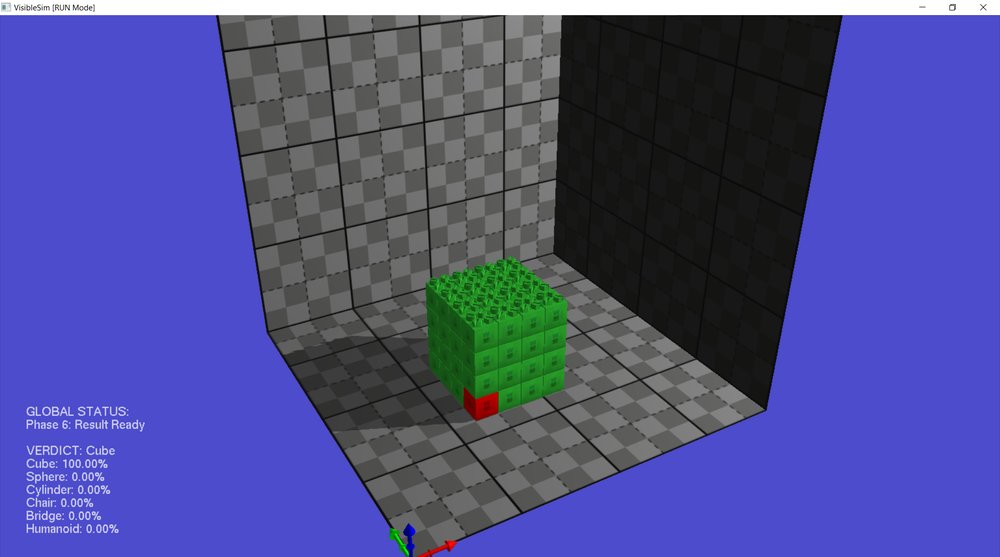
\includegraphics[width=0.3\textwidth]{figures/AI4PM-CNN/AI4PM-DeepEmbedded/sim_cube.png}\hfill
    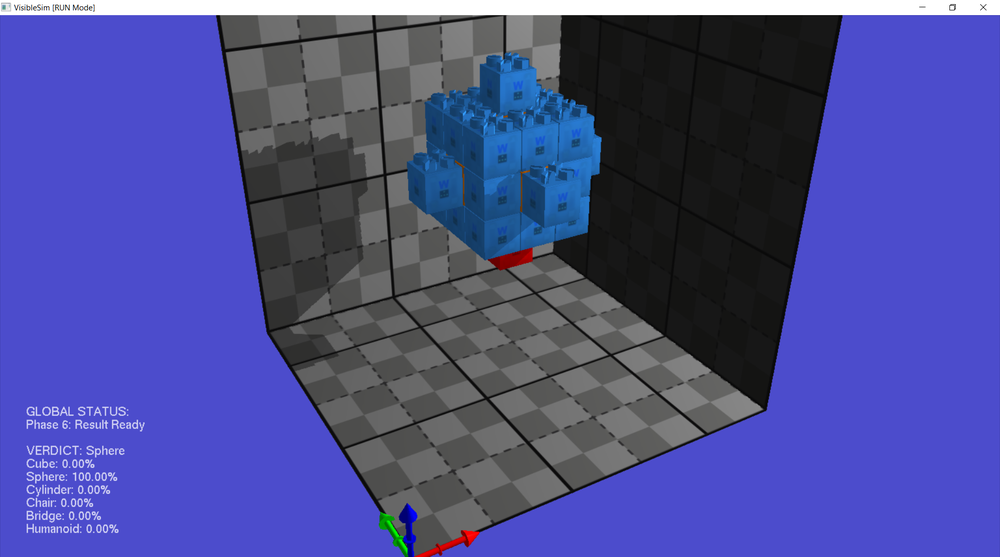
\includegraphics[width=0.3\textwidth]{figures/AI4PM-CNN/AI4PM-DeepEmbedded/sim_sphere.png}\hfill
    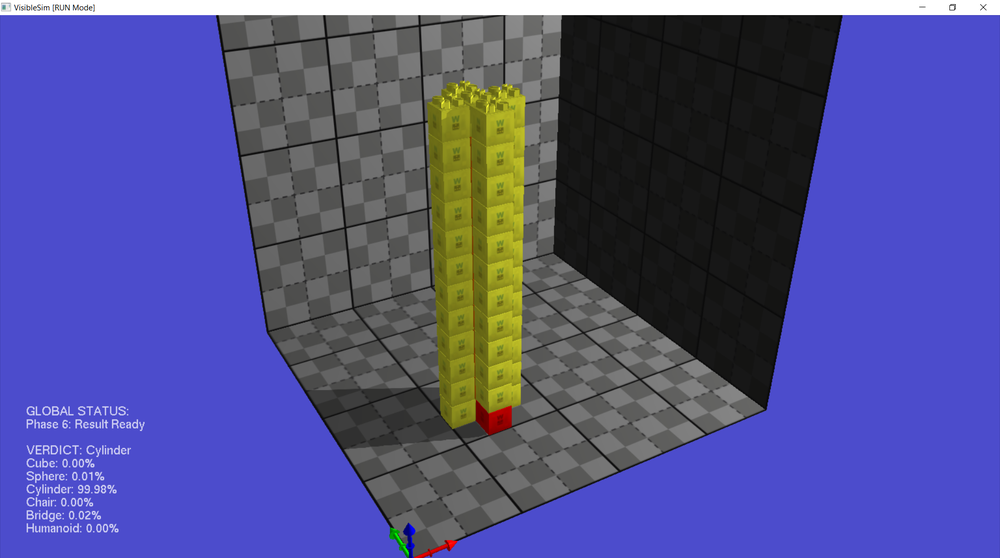
\includegraphics[width=0.3\textwidth]{figures/AI4PM-CNN/AI4PM-DeepEmbedded/sim_cylinder.png}\\[2mm]
    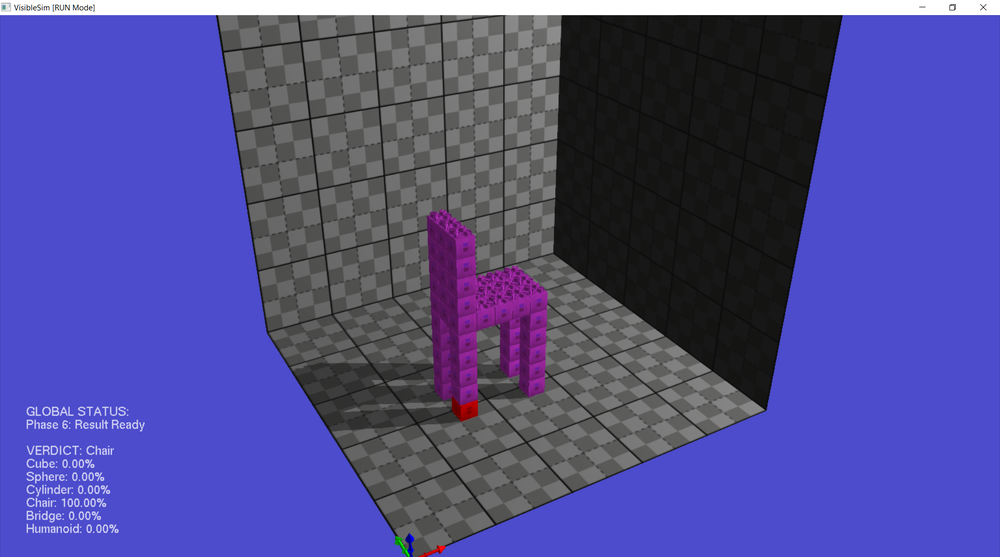
\includegraphics[width=0.3\textwidth]{figures/AI4PM-CNN/AI4PM-DeepEmbedded/sim_chair.png}\hfill
    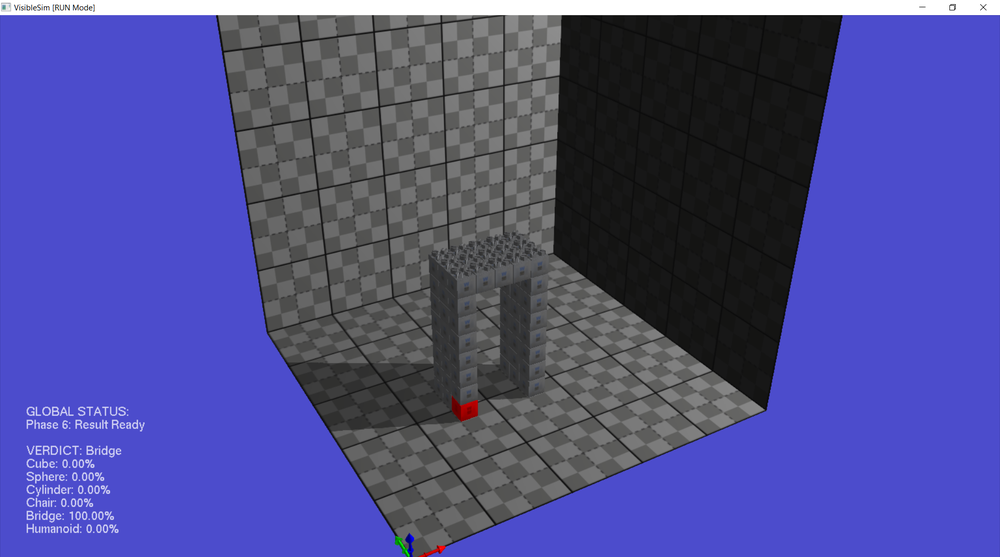
\includegraphics[width=0.3\textwidth]{figures/AI4PM-CNN/AI4PM-DeepEmbedded/sim_bridge.png}\hfill
    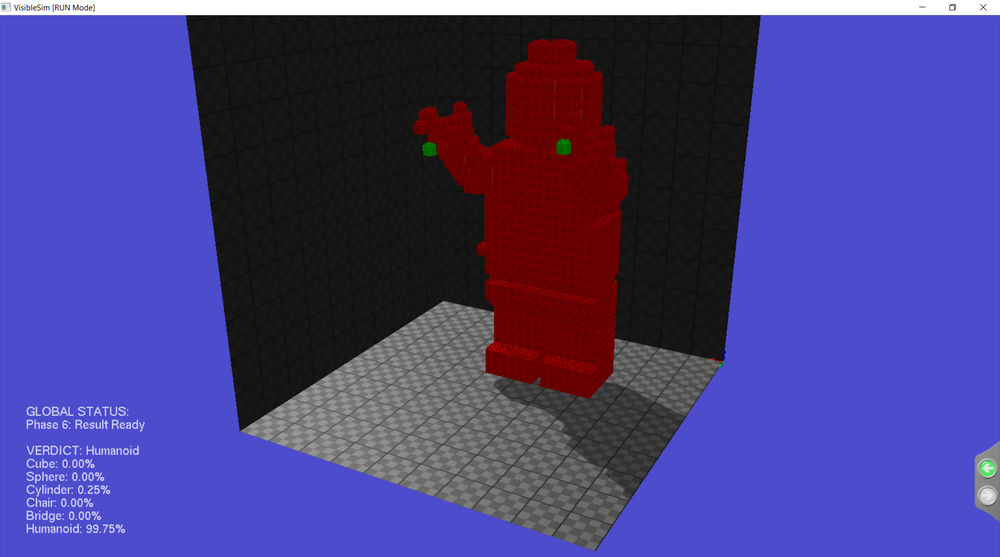
\includegraphics[width=0.3\textwidth]{figures/AI4PM-CNN/AI4PM-DeepEmbedded/sim_humanoid.png}
    \caption{VisibleSim classification results for all six shape classes, Stage 6 model. Top row, left to right: Cube, Sphere, Cylinder. Bottom row: Chair, Bridge, Humanoid.}
    \label{fig:sim-shapes}
\end{figure}

\section{Real Hardware Results (Final Model)}

We tested the quantized model on real BlinkyBlocks hardware for all six shape classes, varying shape size, rotation, translation, and scale for each class as described in Section~5.1. The accuracy per class is summarized in Table~\ref{tab:hw-results} and shown in Figure~\ref{fig:accuracy-hw}. Sphere and Cylinder were classified perfectly, both reaching 100.0\% accuracy across every variation tested, followed by Cube at 85.0\%, Chair at 80.0\%, and Humanoid also at 80.0\%; Bridge was the weakest class at 73.3\%. The overall accuracy across all classes and configurations was 88.0\%.

\begin{table}[H]
    \centering
    \caption{Real BlinkyBlocks hardware classification accuracy by shape, Stage 6 model.}
    \label{tab:hw-results}
    \begin{tabular}{lcc}
        \toprule
        Shape & Correct / Total & Accuracy \\
        \midrule
        Cube      & --/20 & 85.0\% \\
        Sphere    & --/20 & 100.0\% \\
        Cylinder  & --/20 & 100.0\% \\
        Chair     & --/15 & 80.0\% \\
        Bridge    & --/15 & 73.3\% \\
        Humanoid  & --/10 & 80.0\% \\
        \bottomrule
    \end{tabular}
\end{table}

\begin{figure}[H]
    \centering
    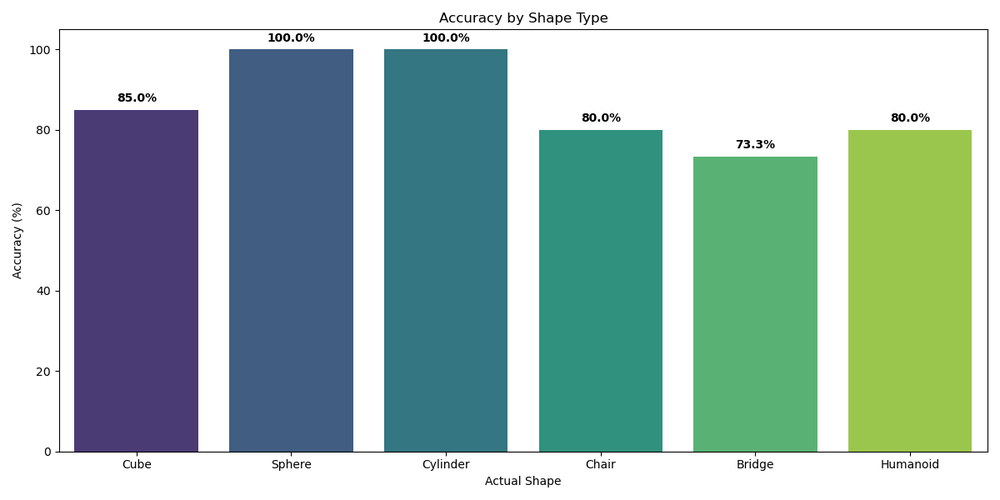
\includegraphics[width=0.6\textwidth]{figures/AI4PM-CNN/AI4PM-DeepEmbedded/hw_accuracy_by_shape.png}
    \caption{Per-class classification accuracy of the quantized Stage 6 model on real BlinkyBlocks hardware.}
    \label{fig:accuracy-hw}
\end{figure}

Figure~\ref{fig:hardware-photos} shows the real BlinkyBlocks platform correctly classifying four of the six shape classes, each block lighting up in the color corresponding to the predicted class (Cube: green, Sphere: blue, Cylinder: yellow, Chair: magenta).

\begin{figure}[H]
    \centering
    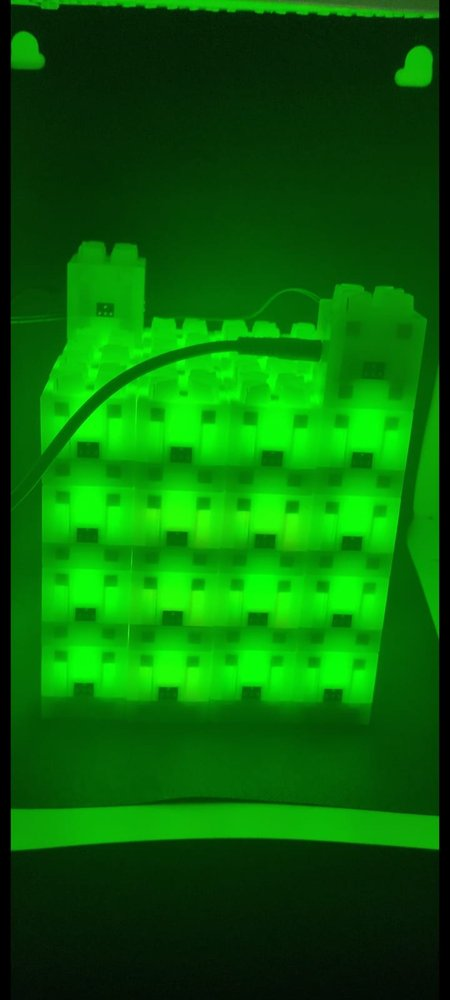
\includegraphics[height=4.5cm,keepaspectratio]{figures/AI4PM-CNN/AI4PM-DeepEmbedded/hw_cube.jpeg}\hfill
    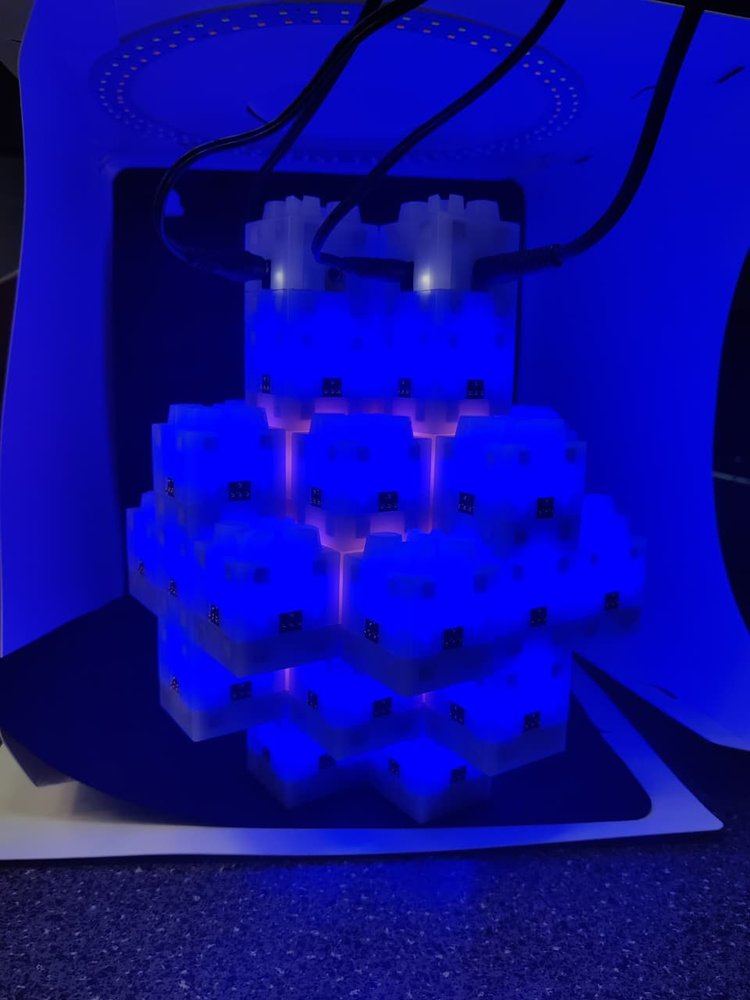
\includegraphics[height=4.5cm,keepaspectratio]{figures/AI4PM-CNN/AI4PM-DeepEmbedded/hw_sphere.jpeg}\hfill
    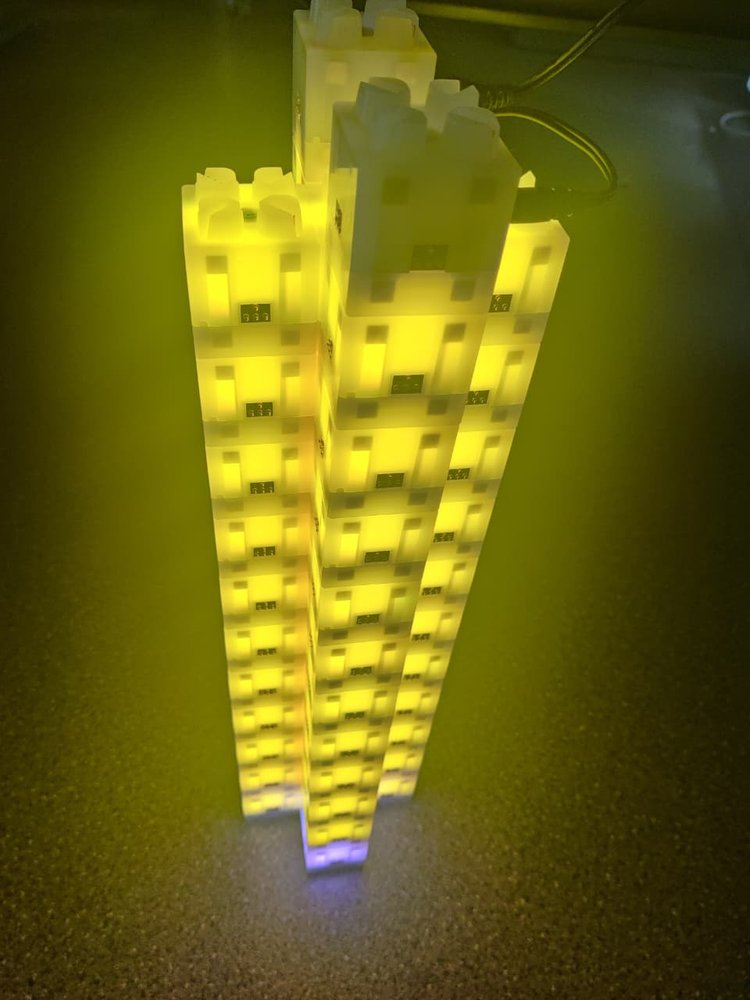
\includegraphics[height=4.5cm,keepaspectratio]{figures/AI4PM-CNN/AI4PM-DeepEmbedded/hw_cylinder.jpeg}\hfill
    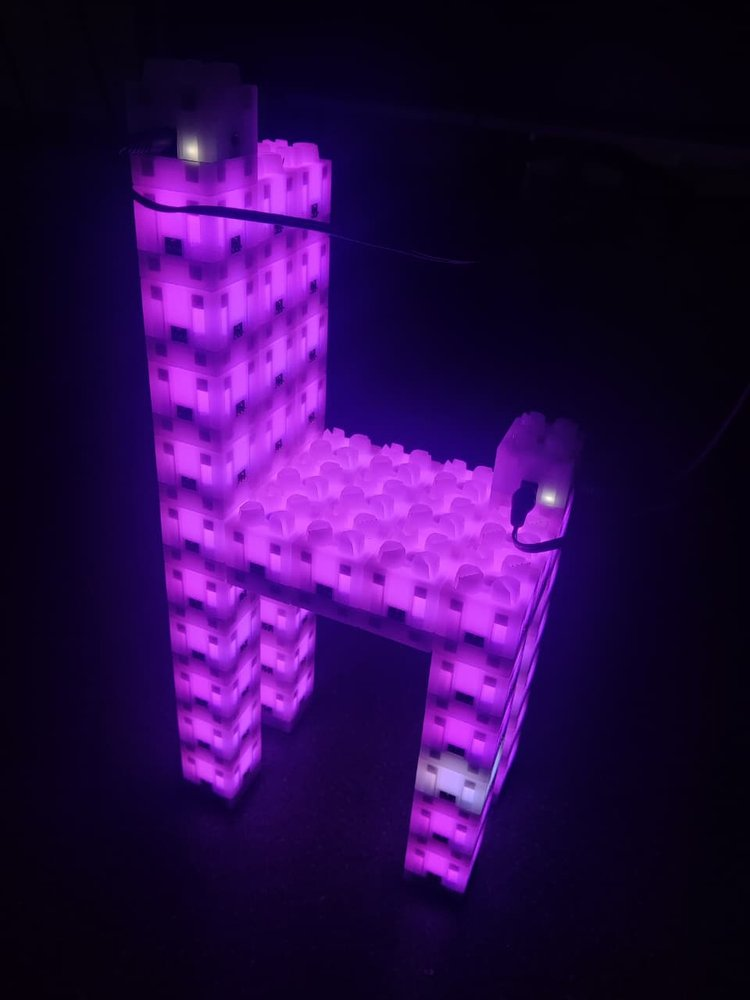
\includegraphics[height=4.5cm,keepaspectratio]{figures/AI4PM-CNN/AI4PM-DeepEmbedded/hw_chair.jpeg}
    \caption{Real BlinkyBlocks hardware running the Stage 6 distributed 3D CNN shape classifier. Left to right: Cube (green), Sphere (blue), Cylinder (yellow), Chair (magenta).}
    \label{fig:hardware-photos}
\end{figure}

\section{Discussion}

The boundaries of the strongest classes (Sphere and Cylinder) are smooth and mostly convex, with no thin protruding structures, whereas the weakest class, Bridge, has thin pillars and a narrow deck that is just one BlinkyBlock wide in some areas. This pattern matches the fact that a real BlinkyBlock can only directly sense occupancy at its 6 face-connected neighbors and must infer the rest of the diagonal cells of its local window, which is more likely to cause errors for thin structures rather than solid and convex ones. When compared to Piranda et al.~\cite{piranda2024ai4pm} for their simpler 3-class shapes and 2D task, our overall accuracy of 88.0\% over 6 3D classes, tested against a wider range of geometric shapes rather than a single fixed configuration per class, is showing the increased difficulty of the demanding task.

This same convex-versus-thin-structure pattern is visible, in embryonic form, as far back as Stage~2 (Section~\ref{sec:stage2}), where the flat ANN's strongest class, Cylinder, was also its most axis-aligned, extruded, and least thin-featured shape, while its weaker classes (Sphere, Cube) already showed lower confidence even without any thin protruding structures at all, suggesting that convex, axis-friendly shapes have been comparatively easy for every architecture in this progression, while genuinely thin or irregular structures have consistently been the harder case, right through to Stage~6's real-hardware evaluation. Unlike the earlier stages, however, Stage~6's per-class accuracy figures come from dozens of size, rotation, translation, and scale variations per class on real hardware rather than a single VisibleSim instance, which makes Bridge's 73.3\% a considerably more demanding standard to meet than any single-instance result reported for Stages~1 through~5.

The gap between Stage~6's VisibleSim results (Table~\ref{tab:sim-results}, all six classes at or above 99.7\% confidence) and its real-hardware results (Table~\ref{tab:hw-results}, overall accuracy 88.0\%, with Bridge as low as 73.3\%) is itself worth examining, since it is the largest sim-to-real gap observed at any stage in this thesis. VisibleSim's simulated communication is idealized: messages between face-connected blocks are delivered without loss and without the timing jitter a real wireless or wired short-range link might introduce, and every simulated block senses its neighbors' occupancy with perfect reliability. Real BlinkyBlocks hardware does not offer these same guarantees unconditionally, and Section~5.4's convex-versus-thin-structure explanation should be understood as one contributing factor among potentially several real-hardware effects (sensing noise, message timing, physical assembly tolerances) that VisibleSim's idealized simulation does not, by construction, reproduce. Disentangling these effects more precisely than this thesis does was outside its scope, but is noted as a natural direction for follow-up work in Chapter~\ref{ch:conclusion}.

\chapter{Contribution to the Problem Statement}
\label{ch:contribution}

Chapter~1 identified two requirements the problem addressed by this internship had to satisfy simultaneously: a distributed architecture capable of classifying a richer vocabulary of volumetric 3D shapes without the combinatorial message-count blow-up exhibited by a naive flat-ANN extension to 3D, and a model small enough, once trained, to be compressed into a real BlinkyBlock's flash memory budget rather than existing only as a VisibleSim simulation.

The results presented in Chapter~\ref{ch:results} show that Stage~6, the Deep Embedded 3D CNN with TinyML int8 quantization, satisfies both requirements concretely, not merely in principle. On the first requirement, message counts across the six-class evaluation (Table~\ref{tab:sim-results}) scale linearly with the number of blocks in the structure being classified, 404 messages for a 47-block Chair and 53,454 messages for a 2835-block Humanoid, rather than exploding combinatorially the way Stage~2's flat 3D ANN did (2.15 to 5.00 million messages for structures of only 704 to 828 blocks, Section~\ref{sec:stage2}). This is a direct, measured resolution of the scaling problem identified in Section~1.2: the same convolutional, locally-computed design principle that produced Stage~3's 68x message-count reduction over Stage~1 (Section~\ref{sec:stage3}) carries through, one additional convolutional phase and three additional shape classes later, to Stage~6's six-class model.

On the second requirement, Table~\ref{tab:quantization} shows the trained Stage~6 model compressed from 67.1 KB to 17.8 KB via int8 weight quantization, a 3.77x reduction, using the same post-training quantization methodology first exercised at Stage~1 on Piranda et al.'s original ANN (Section~\ref{sec:stage1}). This compressed model is not a simulation-only artifact: Chapter~\ref{ch:results}'s real-hardware evaluation (Table~\ref{tab:hw-results}) confirms an overall accuracy of 88.0\% across all six classes when the quantized weights are actually flashed onto physical BlinkyBlocks and evaluated under real sensing and communication conditions, rather than VisibleSim's idealized message delivery.

The contribution is not, however, a complete or final solution to every aspect of the problem as originally stated. Bridge, the shape class with the thinnest and sparsest structure among the six trained, remains the weakest at 73.3\% real-hardware accuracy (Table~\ref{tab:hw-results}), and the discussion in Section~5.4 traces this weakness to a specific, identifiable cause: BlinkyBlocks can only directly sense occupancy at their six face-connected neighbors, and must infer the remaining diagonal cells of their local $3\times3\times3$ window, an inference that is inherently less reliable for thin, sparse structures than for the solid, convex ones (Sphere, Cylinder) the architecture handles best. This limitation is a property of the sensing model shared by every stage in this thesis's progression, not something the Stage~6 architecture change alone can resolve, and is addressed as a direction for future work in Chapter~\ref{ch:conclusion}.

It is also worth stating explicitly what this contribution does \emph{not} claim. It does not claim that the Deep Embedded 3D CNN of Stage~6 is the only architecture capable of satisfying the two requirements above, nor that three convolutional phases and six shape classes represent some fundamental limit of what this general design family can achieve; Section~\ref{ch:conclusion}'s perspectives discuss directly how both the depth and the shape vocabulary could plausibly be extended further using the same underlying communication pattern. What this chapter's evidence does support is a narrower, more defensible claim: that the specific problem stated in Chapter~1, richer 3D shape classification without a flat architecture's message-count explosion and deployable within a real BlinkyBlock's memory budget, has a working, measured, hardware-validated solution, and that the six-stage methodology of Chapter~\ref{ch:methodology} documents, with evidence at every step, why that solution takes the specific architectural form it does rather than any of the five alternative designs tried and set aside along the way.

\chapter{Conclusion and Perspectives}
\label{ch:conclusion}

\section{Conclusion}

This thesis documented an internship carried out at institut FEMTO-ST that set out to extend Piranda et al.'s demonstration of a distributed Artificial Neural Network on BlinkyBlocks toward richer, volumetric 3D shape recognition, while keeping every resulting model deployable within BlinkyBlocks' strict per-module memory budget. Rather than designing a single architecture directly, the work proceeded through six successive stages, each diagnosed for a specific limitation that motivated the next: an int8-quantized reproduction of Piranda et al.'s original 2D ANN (Stage~1); a naive 3D extension of that same flat architecture, whose message count exploded into the millions (Stage~2); a 2D CNN using local, face-neighbor message passing, which reduced message count by roughly 68x under matched conditions (Stage~3); a 3D CNN relying on a hardcoded height-map projection, which extended that efficiency to 3D shapes but reintroduced a fixed, orientation-dependent role for only some blocks (Stage~4); a fully Embedded 3D CNN in which every block participates equally, with message count now genuinely proportional to block count (Stage~5); and finally a Deep Embedded 3D CNN with three convolutional phases and six shape classes, compressed with TinyML int8 quantization (Stage~6).

We worked on a distributed 3D Convolutional Neural Network for module shape classification on Programmable Matter systems, extending the message-passing, agent-based approach of Piranda et al.~\cite{piranda2024ai4pm} from a flat ANN over simple, fixed 2D configurations to a deeper architecture capable of classifying six classes. To fit the model within the flash memory budget of a BlinkyBlock, we applied TinyML weight quantization, converting the trained weights from float32 to int8 and reducing model size by 3.77 times with no change to the message format. We validated the model both in the VisibleSim simulator and on a real BlinkyBlocks platform, getting an overall accuracy of 88.0\% across all six classes, with per-class accuracy ranging from 73.3\% (Bridge) to 100\% (Sphere and Cylinder).

Chapter~\ref{ch:results}'s comparative summary across all six stages (Table~\ref{tab:comparative}) makes explicit what each stage in this progression contributed and what it left unresolved, and Chapter~\ref{ch:contribution} traced these results back to the specific problem statement of Chapter~1, concluding that the final Stage~6 model resolves both the message-scaling and the memory-footprint requirements concretely and measurably, while leaving thin-structure sensing accuracy (exemplified by Bridge) as an open limitation rather than a fully solved problem.

\section{Perspectives}

Several directions for future work follow directly from the limitations identified across this thesis's six stages. Thin, sparse shapes like the Bridge remain the hardest case, since a real BlinkyBlock can only directly sense its 6 face-connected neighbors; closing this gap, alongside expanding the shape vocabulary and testing on larger and more diverse real BlinkyBlocks assemblies, is left as future work. A more direct sensing mechanism, or a training procedure that explicitly accounts for the diagonal-cell inference error described in Section~5.4, could narrow the gap between Bridge's real-hardware accuracy and the near-perfect figures achieved on Sphere and Cylinder. Beyond the six shape classes evaluated in this thesis, the same Stage~6 architecture places no fundamental limit on class count beyond the final fully-connected layer's output size, suggesting that a considerably richer shape vocabulary could be trained without further architectural change, provided sufficient labeled training data is generated. Finally, on-device training, briefly noted as a future direction by Piranda et al.~\cite{piranda2024ai4pm} for their own architecture, remains an open question for the deeper, convolutional architecture developed in this thesis, and would represent a further step toward Programmable Matter systems capable of adapting their own shape-recognition capability without any offline training step at all.

Beyond these directions raised directly by Stage~6's limitations, the sim-to-real gap discussed in Section~5.4 also points toward a methodological direction worth pursuing independently of any specific architectural change: training the model against occupancy data that more closely reflects what a real BlinkyBlock can actually sense (its own state and that of its 6 face neighbors only), rather than against VisibleSim's idealized full local neighborhood, could in principle narrow the accuracy gap between simulated and real-hardware evaluation without requiring any change to the message-passing architecture itself. More broadly, the comparative methodology followed throughout Chapter~\ref{ch:methodology}, implement, measure message count and accuracy, diagnose the specific limitation, and design the next stage to directly test whether that limitation has been resolved, is not specific to shape recognition and could plausibly be applied to other distributed learning tasks on BlinkyBlocks or similar lattice-based Programmable Matter platforms, such as distributed defect detection, self-assembly verification, or collaborative sensing tasks that share the same fundamental constraint of purely local computation and communication that has shaped every design decision in this thesis.

\begin{thebibliography}{9}

\bibitem{piranda2024ai4pm}
B. Piranda, M. A. Nemer, A. Makhoul, and J. Bourgeois,
``AI4PM: Distributed and Intelligent Programmable Matter,''
2024.

\bibitem{dobreva}
K. Dobreva et al.,
``Distributed control of pivoting cube modular robots via convolutional message passing,''
2023.

\bibitem{capogrosso}
L. Capogrosso et al.,
``A survey on quantization for embedded neural network inference,''
2024.

\bibitem{somvanshi}
S. Somvanshi et al.,
``TinyML and TinyDL: A survey on resource-constrained deep learning,''
2024.

\end{thebibliography}

\end{document}
